\documentclass[10pt]{beamer}
\usepackage{amsmath}
\usepackage{amssymb}
%\usepackage{dsfont}
\usepackage{accents}
\usepackage{hyphenat}
\usepackage{multirow}
\usepackage{animate}
\usetheme[progressbar=frametitle]{metropolis}
\setbeamercolor{background canvas}{bg=white}
% \usetheme{focus}
\usepackage{appendixnumberbeamer}
\usefonttheme[onlymath]{serif}
\usepackage{booktabs}
\usepackage[scale=2]{ccicons}

\usepackage{pgfplots}
\usepgfplotslibrary{dateplot}

\usepackage{xspace}
\newcommand{\themename}{\textbf{\textsc{metropolis}}\xspace}
\usetikzlibrary{snakes,arrows,mindmap,trees,backgrounds,shapes.geometric,calc}
\tikzset{graphics/.style={inner sep=0,outer sep=0}}
\tikzset{scaleall/.style={scale=#1, transform shape}}
\usepgflibrary{arrows}


\newlength{\bbw}
\newlength{\bbh}
\newcommand{\pcuad}[3][]{
  % First arguments is an optional prefix for the coordinate names

  \setlength{\bbw}{#2}
  \setlength{\bbh}{#3}
  \useasboundingbox(0,0) rectangle (\bbw,\bbh);

  \path(.5\bbw,.5\bbh) coordinate(#1cp);
  \path(\bbw,0)        coordinate(#1se);
  \path(0,0)           coordinate(#1sw);
  \path(0,\bbh)        coordinate(#1nw);
  \path(\bbw,\bbh)     coordinate(#1ne);
 
  
  \path(\bbw,.5\bbh) coordinate(#1ep);
  \path(.5\bbw,0)    coordinate(#1sp);
  \path(.5\bbw,\bbh) coordinate(#1np);
  \path(0,.5\bbh)    coordinate(#1wp);
       
  \path(.75\bbw,.5\bbh) coordinate(#1hr);
  \path(.25\bbw,.5\bbh) coordinate(#1hl);
  \path(.5\bbw,.25\bbh) coordinate(#1vl);
  \path(.5\bbw,.75\bbh) coordinate(#1vu);

  \path(.75\bbw,.75\bbh) coordinate(#1c1);
  \path(.25\bbw,.75\bbh) coordinate(#1c2);
  \path(.25\bbw,.25\bbh) coordinate(#1c3);
  \path(.75\bbw,.25\bbh) coordinate(#1c4);


%  +-----------------------------------------------+
%  |nw                    np                     ne|
%  |                                               |
%  |                                               |
%  |          c2          vu          c1           |
%  |                                               |
%  |                                               |
%  |wp        hl          cp          hr         ep|
%  |                                               |
%  |                                               |
%  |          c3          vl          c4           |
%  |                                               |
%  |                                               |
%  |sw                    sp                     se|
%  +-----------------------------------------------+
}
 
        
\newcommand{\showcuad}[1][]{

   \draw[help lines,xstep=.5,ystep=.5,gray!10] (#1sw) grid (#1ne);
   \draw[help lines,xstep=1,ystep=1,gray]      (#1sw) grid (#1ne);
   %\draw[help lines,xstep=.25,ystep=.25,gray!20] (sw) grid (ne);
   % \draw[help lines,xstep=1,ystep=1,gray] (sw) grid (ne);
   % \foreach \x in {-20,-14.5,...,20} {
   %     \node [anchor=north, gray,yshift=30] at (\x,0) {\tiny \bf \x};
   %     \node [anchor=east,gray,xshift=30] at (0,\x) {\tiny \bf  \x};
   % }
               
    \fill(#1se) circle(.1) node[anchor=south east]{#1se};
    \fill(#1sw) circle(.1) node[anchor=south west]{#1sw};
    \fill(#1ne) circle(.1) node[anchor=north east]{#1ne};
    \fill(#1nw) circle(.1) node[anchor=north west]{#1nw};
                  
    \fill(#1hr) circle(.1) node[above]{#1hr};
    \fill(#1hl) circle(.1) node[above]{#1hl};
    \fill(#1vu) circle(.1) node[above]{#1vu};
    \fill(#1vl) circle(.1) node[above]{#1vl};
                  
    \fill(#1sp) circle(.1) node[anchor=south]{#1sp};
    \fill(#1wp) circle(.1) node[anchor=west] {#1wp};
    \fill(#1np) circle(.1) node[anchor=north]{#1np};
    \fill(#1ep) circle(.1) node[anchor=east] {#1ep};

    \fill(#1cp) circle(.1) node[above]{#1cp};
    \fill(#1c1) circle(.1) node[above]{#1c1};
    \fill(#1c2) circle(.1) node[above]{#1c2};
    \fill(#1c3) circle(.1) node[above]{#1c3}; 
    \fill(#1c4) circle(.1) node[above]{#1c4};

    %\fill[red](cp|-c1) circle(.1) node[anchor=north]{cp|-c1};

}

\newcommand{\ds}{\displaystyle}
\newcommand{\dsum}{\displaystyle \sum}
\newcommand{\uu}[1]{{\boldsymbol #1}}
\newcommand{\ud}{\,\mathrm{d}}
\def\ttau{\uu{\tau}}
\def\bb{\uu{b}}
\def\nb{\uu{n}}
\def\pb{\uu{p}}
\def\wb{\uu{w}}
\def\xb{\uu{x}}
\def\ab{\uu{a}}
\def\mb{\uu{m}}
\def\yb{\uu{y}}
\def\vb{\uu{v}}
\def\fb{\uu{f}}
\def\zb{\uu{z}}
\def\Xb{\uu{X}}
\def\etab{\uu{\eta}}
\def\thetab{\uu{\theta}}
\def\lambdab{\uu{\lambda}}
\def\gammab{\uu{\gamma}}
\def\taub{\uu{\tau}}
\def\varphib{\uu{\varphi}}
\def\Ab{\uu{A}}
\def\Bb{\uu{B}}
\def\Gb{\uu{G}}
\def\Fb{\uu{F}}
\def\Jb{\uu{J}}
\def\Rb{\uu{R}}
\def\Tb{\uu{T}}
\def\rb{\uu{r}}
\def\ab{\uu{a}}
\newcommand{\molar}[1]{\underaccent{\bar}{#1}}
\def\um{\molar{U}}
\def\hm{\molar{H}}
\def\sm{\molar{S}}
\def\am{\molar{A}}
\def\gm{\molar{G}}
\def\hh{\hat{H}}
\def\sh{\hat{S}}
\def\vm{\molar{V}}
\def\cp{C_{\rm P}}
\def\cv{C_{\rm V}}
\def\cps{C_{\rm P}^*}
\def\cvs{C_{\rm V}^*}
\def\wsd{\dot{W}_s}
\def\md{\dot{M}}\newcommand{\pd}[2]{\left(\frac{\partial {#1}}{\partial 
{#2}}\right)}
\newcommand{\tpd}[3]{\left(\frac{\partial {#1}}{\partial {#2}}\right)_{#3}}
\newcommand{\tpdn}[4]{\left(\frac{\partial^{#4} {#1}}{\partial 
{#2}^{#4}}\right)_{#3}}



\title{Modern Molecular Simulations using Extended-Lagrangian Approaches}
\date{March 25, 2024}
\author{Cameron F. Abrams\\Bartlett '81 -- Barry '81 Professor and Head\\cfa22@drexel.edu}
\institute{Drexel University, Department of Chemical and Biological Engineering}
\titlegraphic{\hfill
\includegraphics[height=0.75cm]{drexel-horz-blue.png}}

\begin{document}

\maketitle

\begin{frame}{Outline}
  \setbeamertemplate{section in toc}[sections numbered]
  \tableofcontents[hideallsubsections]
\end{frame}

\section{Introduction and Motivation}

\begin{frame}[fragile]{Lengthening the Reach of Molecular Dynamics Simulations}
%\vspace{5mm}
%\hspace{-5mm}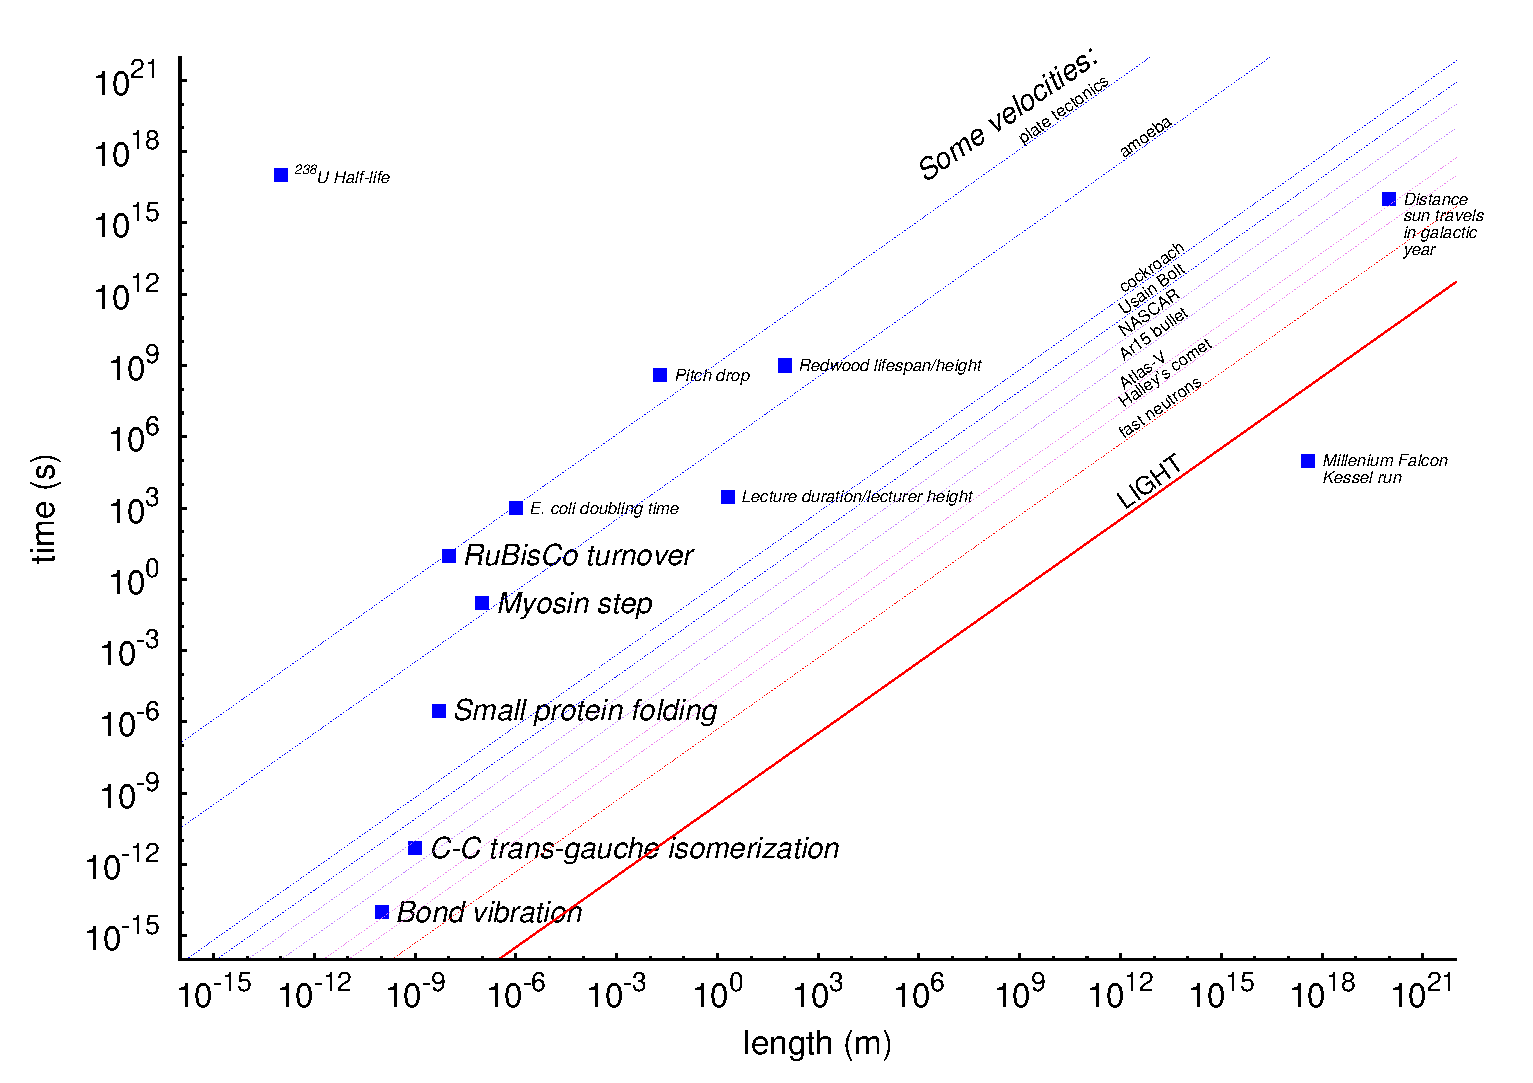
\includegraphics[width=\textwidth]{time_vs_length.eps}
\begin{tikzpicture}[scale=1.5]
\node[anchor=south west,inner sep=0] (image) at (0,0) 
{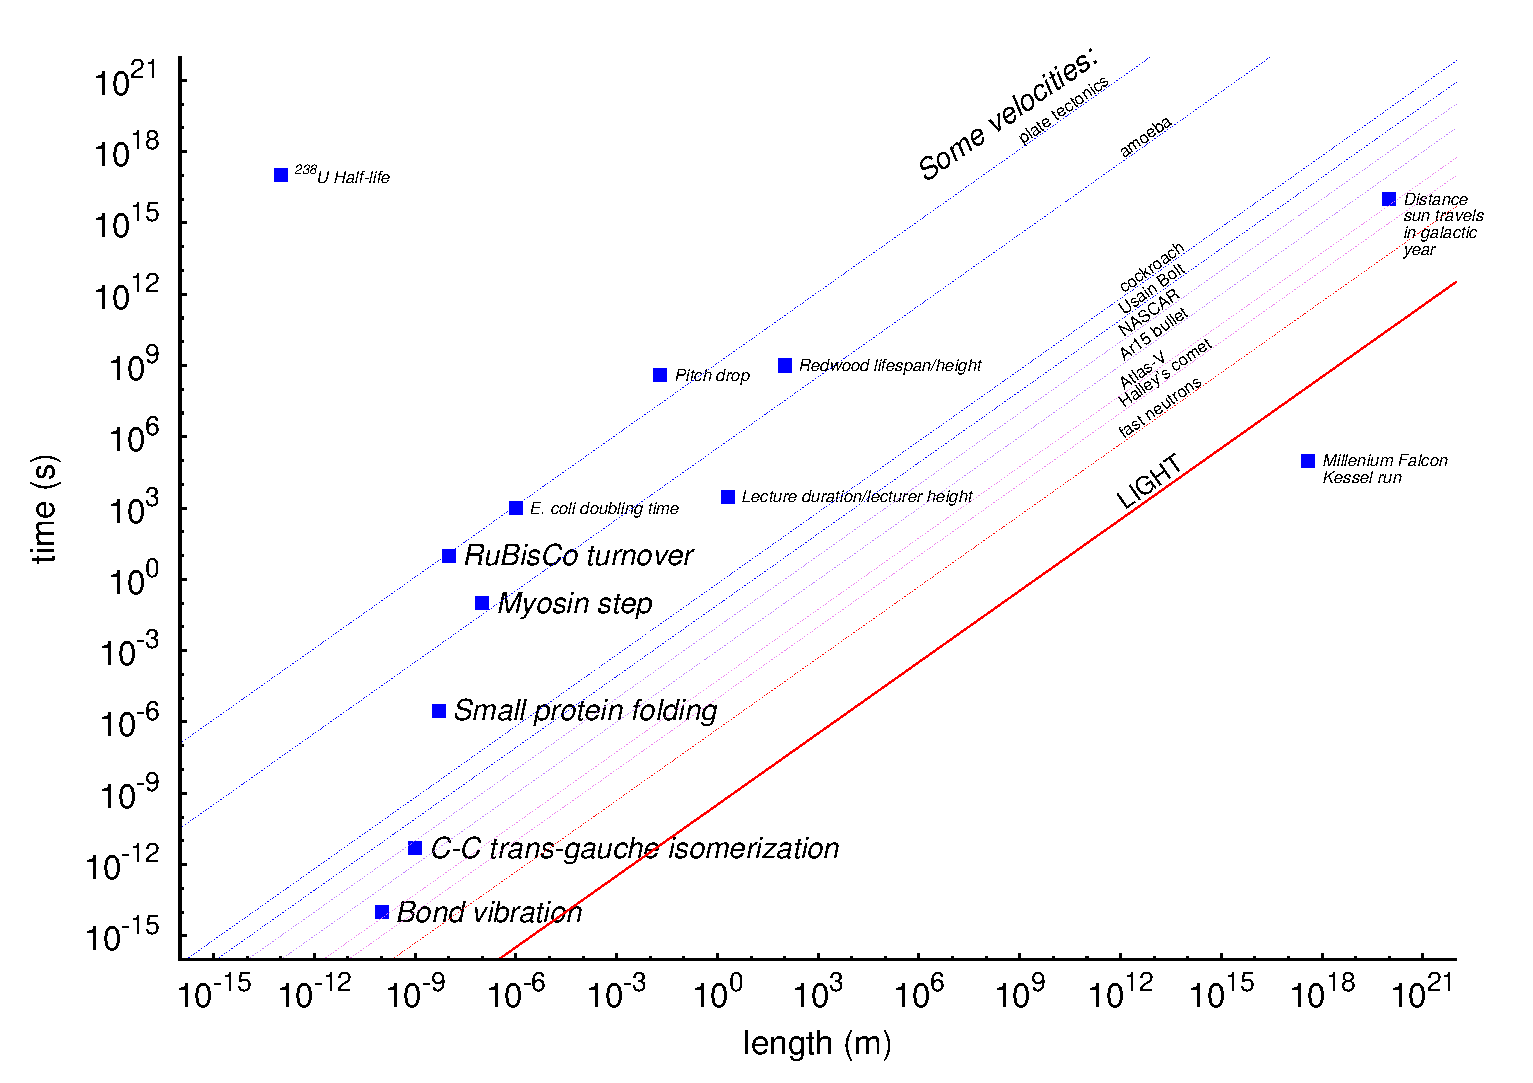
\includegraphics[width=0.975\textwidth]{time_vs_length.eps}};
\begin{scope}[x={(image.south east)},y={(image.north west)}]
\draw[red,thick,rounded corners] (0.2,0.125) rectangle (0.32,0.375);
\draw[red,thick] (0.26,0.275) node {MD};
\draw[->, green!80!black, thick, snake=snake, segment amplitude=.4mm, segment length=2mm, 
line after snake=1mm] (0.29,0.375) -- (0.29,0.45);
\draw[->, green!80!black, thick, snake=snake, segment amplitude=.4mm, segment length=2mm, 
line after snake=1mm] (0.26,0.375) -- (0.26,0.475);
\draw[->, green!80!black, thick, snake=snake, segment amplitude=.4mm, segment length=2mm, 
line after snake=1mm] (0.23,0.375) -- (0.23,0.5);
\draw[->, blue!80!white, thick, snake=snake, segment amplitude=.4mm, segment length=2mm, 
line after snake=1mm] (0.32,0.285) -- (0.38,0.285);
\draw[->, blue!80!white, thick, snake=snake, segment amplitude=.4mm, segment length=2mm, 
line after snake=1mm] (0.32,0.25) -- (0.4,0.25);
\node[green!80!black,text width=2cm,rotate=90] at (0.25,0.65) {Enhanced sampling};
%\draw [red,thick,rotate=-90] (0.3,0.6) node {Enhanced Sampling};
\draw [blue!80!white,thick] (0.57,0.27) node {Resolution coarsening};
\end{scope}
\end{tikzpicture}
\end{frame}



\tikzstyle{startstop} = [rectangle, rounded corners, minimum width=1cm, minimum height=0.5cm,text centered, draw=black, fill=red!30]
\tikzstyle{io} = [trapezium, trapezium left angle=70, trapezium right angle=110, minimum width=1cm, minimum height=0.5cm, text centered, draw=black, fill=blue!30]
\tikzstyle{process} = [rectangle, minimum width=1cm, minimum height=1cm, text centered, draw=black, fill=orange!30]
\tikzstyle{decision} = [diamond, minimum width=1cm, minimum height=1cm, text centered, draw=black, fill=green!30]
\tikzstyle{myarrow} = [thick,->,>=stealth]
\begin{frame}[fragile]{Molecular Dynamics (MD)}
\begin{tikzpicture}[scaleall=1.0,node distance=2cm]
\node (start) [startstop] {Start};
\node (init) [io,right of=start,xshift=1cm,text width=2cm] {Initial atomic positions and velocities};
\node (force) [process,right of=init,xshift=1cm] {Get forces};
\node (integrate) [process,below of=force] {Update positions and velocities};
\node (check) [decision,below of=integrate] {Done?};
\node (continue) [process,right of=check,xshift=1cm] {\begin{tabular}{c} Update time \\ by 10$^{-15}$ s \end{tabular}};
\node (terminate) [process,left of=check,xshift=-1cm] {Save data};
\node (stop) [startstop,left of=terminate] {Stop};
\draw [myarrow] (start) -- (init);
\draw [myarrow] (init) -- (force);
\draw [myarrow] (force) -- (integrate);
\draw [myarrow] (integrate) -- (check);
\draw [myarrow] (check) -- node[anchor=south] {no} (continue);
\draw [myarrow] (continue) |- (force);
\draw [myarrow] (check) -- node[anchor=south] {yes} (terminate);
\draw [myarrow] (terminate) -- (stop);
\end{tikzpicture}
\end{frame}


\begin{frame}[fragile]{MD and Ergodicity}

\textcolor{green!80!black}{Statistical mechanics:}
$$
P_\nu = \left\{\begin{array}{l}
    \mbox{Probability of state $\nu \equiv (\xb,\vb)$}\\
    \mbox{out of \textcolor{blue!80!white}{ensemble} of states}\\
    \mbox{at equilibrium}\\
        \end{array}\right\}
$$

Observables as \textcolor{blue!80!white}{ensemble averages}:
$$
\langle G \rangle = \sum_\nu P_\nu G_\nu
$$

\textcolor{green!80!black}{Ergodic hypothesis: Infer $P_\nu$ via uniform random sampling}
$$
\langle G \rangle = \lim_{t\rightarrow\infty} \frac{1}{N}\sum_{i}^{N}G(\nu_{\rm MD}(t_i))
$$ 

\begin{center}
\fbox{\textcolor{red!80!black}{Ergodicity in MD is (usually) unattainable!}}
\end{center}

\end{frame}



\begin{frame}{The Essential Problem: Poor Sampling of Feature Space}
    \begin{tikzpicture}[scaleall=1.0]
    \pcuad{\textwidth}{\textheight}
    \path(nw) ++(-1,-0.5) node(graphic1)[anchor=north west]{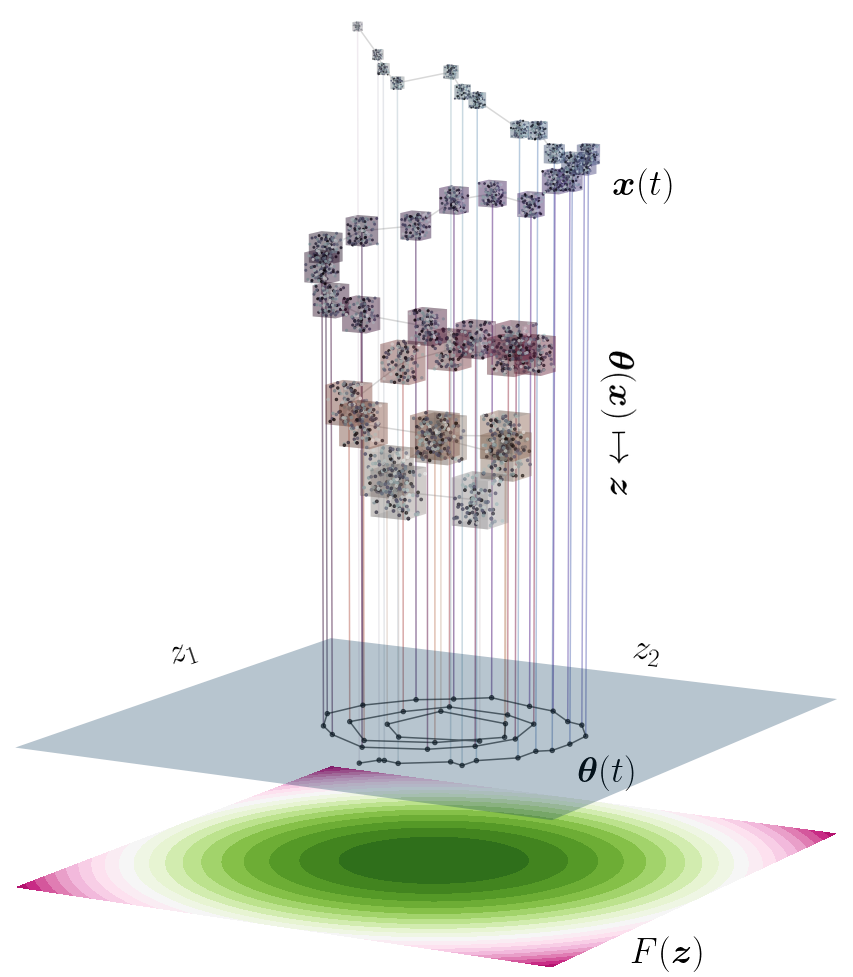
\includegraphics[width=0.6\textwidth]{hmmdfig-crop.png}};
    \path(np) ++(-1,0) node(line1)[anchor=north west]{Configuration space $\xb^{3N} \equiv [(x_0,x_1,x_2)_1,\dots]$}
              ++(0,-1) node(line2)[anchor=west]{MD: $m_i\ddot{x}_i = -\nabla_iV(\xb) + \mbox{ensemble forces}$}
              ++(1,-1) node(line3)[anchor=west]{Samples $\Rightarrow\ \xb(t_1),\ \xb(t_2),\ \dots$}
              ++(0,-1) node(line4)[anchor=west]{Ergodicity: $\displaystyle\langle X\rangle \approx \frac{1}{n_\tau}\sum_{i=1}^{n_\tau} X[\xb(t_i)]$}
              ++(-1.3,-1) node(line5)[anchor=west]{Mapping configuration space}
              ++(0,-0.4) node(line5)[anchor=west]{to feature space}
              ++(0.25,-1.) node(line6)[anchor=west]{Feature space: $\zb^M \equiv (z_1,z_2,\dots)$}
              ++(0,-2) node(line7)[anchor=west]{Free energy: $F(\zb)=-k_{\rm B}T\ln\langle\delta\left[\theta(\xb)-\zb\right]\rangle$};
    \end{tikzpicture}
    \end{frame}
    

\begin{frame}{Extended Lagrangian Formalisms}
\begin{tikzpicture}[scaleall=1.0]
\pcuad{\textwidth}{\textheight}
\path(nw) ++(0,0) node(graphic1)[anchor=north west]{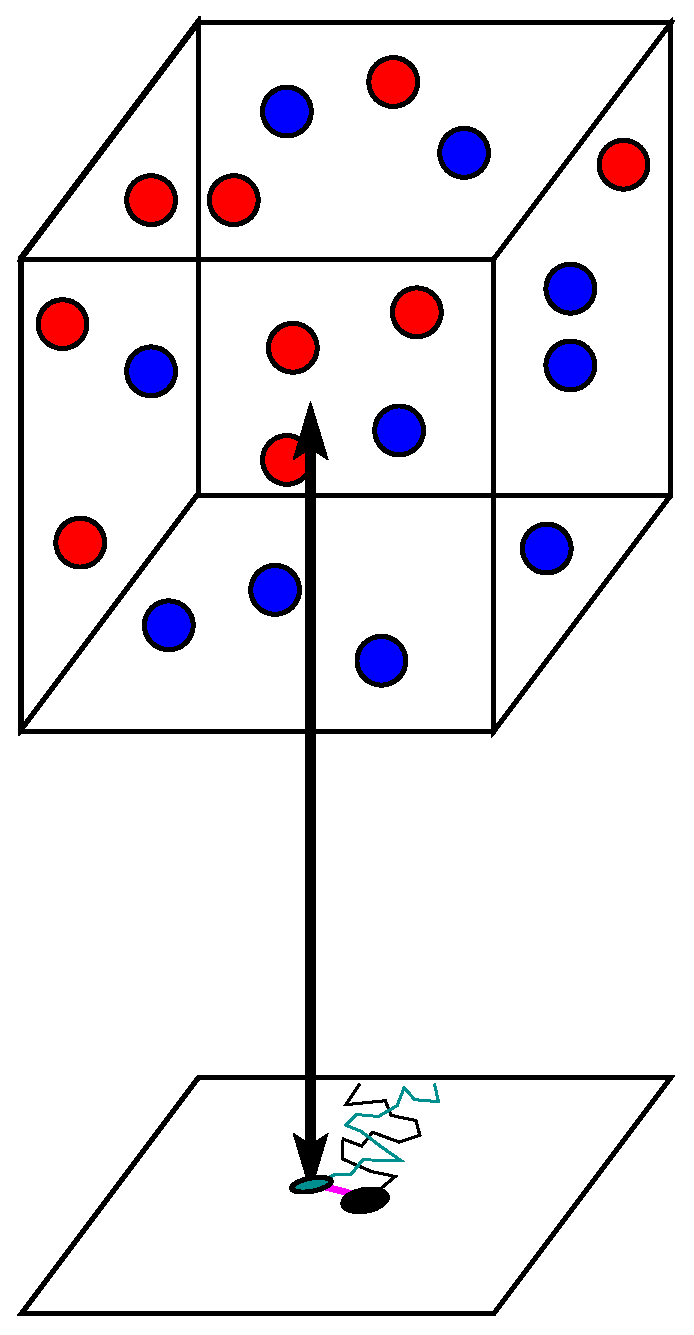
\includegraphics[width=0.35\textwidth]{hmmd-graphic2.eps}};
\path(graphic1) ++(2,3) node(label1)[anchor=north west, text width=0.7\textwidth]{$\displaystyle m_i\ddot{x}_i = -\nabla_iV(\xb)-\sum_{j=1}^M\kappa[\theta_j(\xb)-z_j]\frac{\partial\theta_j}{\partial x_i} + \mbox{e.f.}$};
\path(graphic1) ++(2,-2) node(label3)[anchor=north west, text width=0.7\textwidth]{$\displaystyle\bar{m}_j\ddot{z}_j = \sum_{k=1}^{M} \mathcal{M}_{jk}\kappa[\theta_k(\xb)-z_k] + \mbox{e.f.}$};
\draw[magenta,thick,rounded corners] (6,5) rectangle (9,6);
\draw[magenta,thick] (7.5,5.5) node[align=left] {Forces link $\xb$ and $\zb$};
\draw[thick,rounded corners] (5,3.5) rectangle (10,4.5);
\draw[thick] (7.5,4) node[align=left] {Bias on $\zb$: Enhanced sampling\\of feature space};
\draw[] (1.25,2) node {$\thetab(\xb)$};
\draw[] (2.5,1.75) node {$\zb$};
\end{tikzpicture}
\end{frame}


\section{Temperature-Accelerated MD}

\begin{frame}[fragile]{Temperature-Accelerated MD}
\vspace{-5mm}
\textcolor{blue}{\tiny Maragliano and Vanden-Eijnden, {\it Chem Phys Lett} {\bf 
426}:168 (2006)}

Extended potential energy:\ \ $\displaystyle U(\xb,\zb) = V(\xb) + 
\frac{1}{2}\kappa\sum_{j=1}^{M}[\theta_j(\xb)-z_j]^2$\\
Dynamics of configurational variables $\xb$ (``restrained MD''):
\begin{displaymath}
m_i\ddot{x}_i = -\frac{\partial V(\xb)}{\partial 
x_i}-\kappa\sum_{j=1}^{M}\left[\theta_j(\xb)-z_j\right]\frac{\partial\theta_j}{
\partial x_i}+\mbox{thermostat @ $\beta$}
\end{displaymath}
Dynamics of auxiliary variables $\zb$ with enforced separation of time-scales:
\begin{displaymath}
\bar\gamma\bar{m}_j\dot{z}_j = \kappa\left[\theta_j(\xb)-z_j\right] + 
(\mbox{noise @ $\bar\beta$}) \approx -\frac{\partial F}{\partial z_j} + 
\mbox{noise}
\end{displaymath}

$\zb$ responds to free energy like $\xb$ responds to potential energy.\\
Taking $\bar\beta < \beta$ ($\bar{T} > T$)\ $\Rightarrow$\ enhanced sampling in 
a chosen feature space.

\end{frame}



\begin{frame}[fragile]{TAMD predicts HIV-1 gp120 conformational changes}
\begin{tikzpicture}
\pcuad{\textwidth}{\textheight}
\path(nw) ++(-0.75,0.0) node(text)[anchor=north west,text width=\textwidth]{{\tiny \textcolor{red!80!black}{CFA and E. Vanden-Eijnden {\it PNAS} {\bf 107}:4961 (2010).}}} ++(0,-0.33) node(topfig)[graphics,anchor=north west]{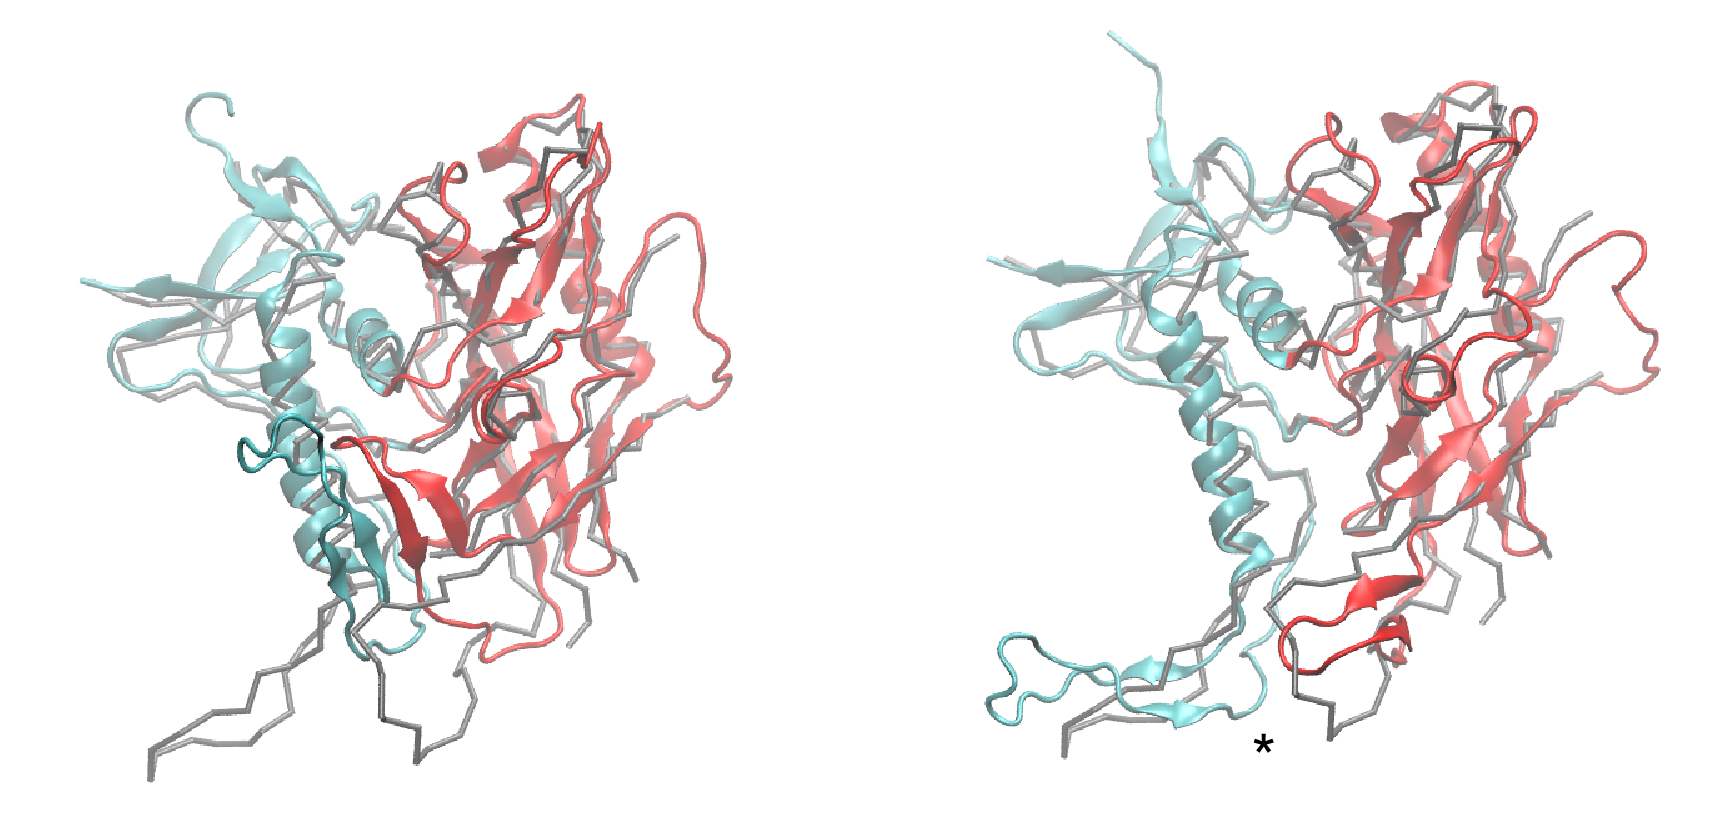
\includegraphics[width=0.8\textwidth]{gp120_snap.png}} ++(0,-4) node(botfig)[graphics,anchor=north west]{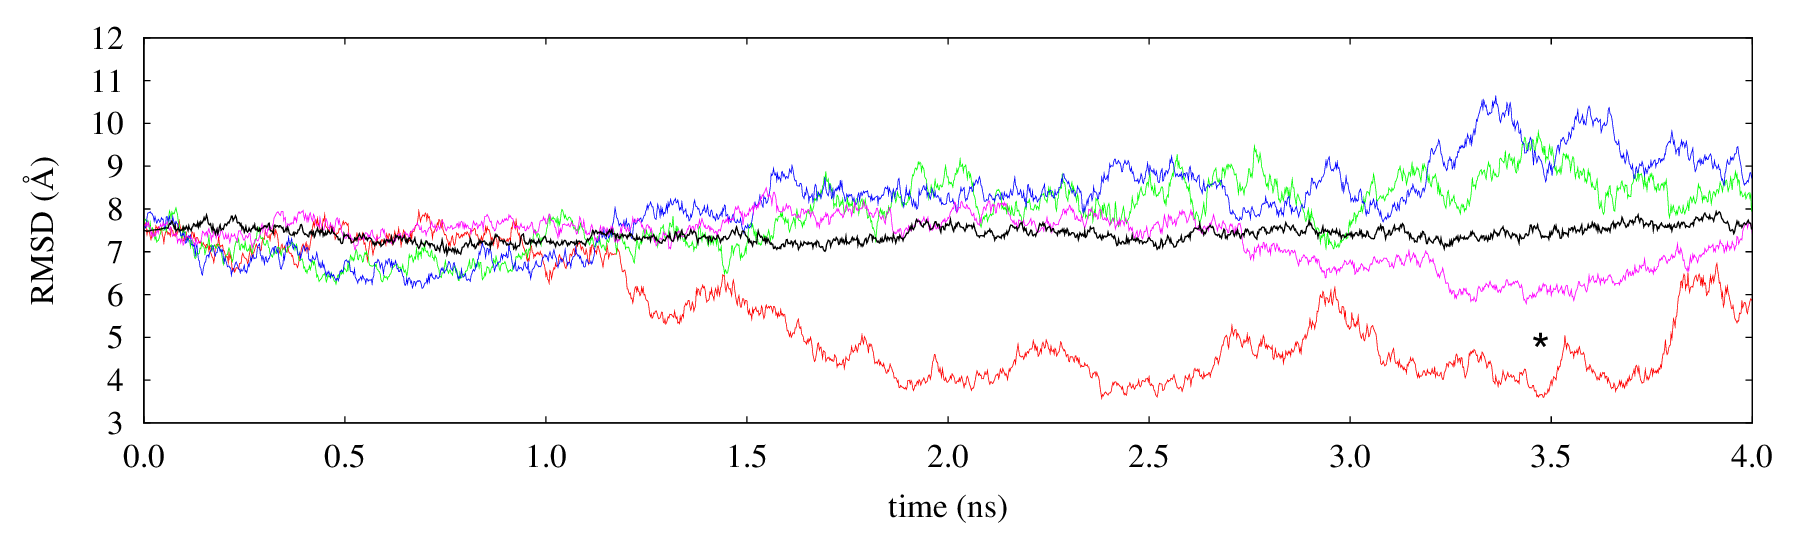
\includegraphics[width=\textwidth]{gp120_rmsdplot.png}}; 
\path(ne) ++(0,0) node(text2)[anchor=north east,text width=0.3\textwidth]{
\begin{itemize}
\item Ribbon: TAMD from 1GC1 (ground state) (\textcolor{teal}{inner}/\textcolor{red}{outer})
\item Tube: Reference from 3HI1 (Ab-F105-bound)
\end{itemize}};
\end{tikzpicture}
\end{frame}



\section{On-the-Fly Parameterization}

\begin{frame}[fragile]{On-the-Fly Parameterization (OTFP) to Get $F$ from TAMD}
    \begin{tikzpicture}
        \pcuad{\textwidth}{\textheight}
        %\showcuad
        \path(se) 
            ++(0,1) node(text)[anchor=south east]{
                {\tiny \textcolor{blue!80!black}{CFA and E. Vanden-Eijnden {\em Chem Phys Lett} {\bf 547}:114 (2012)}}
            };
        \path(nw) 
            ++(0,-0.5) node(text)[anchor=west]{
                \textcolor{blue!80!black}{Basis-function expansion}
            }
            ++(0,-0.75) node(Fz)[anchor=west]{
                $\ds \tilde{F}(\zb) = \sum_k\lambda_k\phi_k(\zb)$
            }
            ++(0,-1) node(text2)[anchor=west]{
                \textcolor{red!80!black}{Error estimate}
            }
            ++(0,-0.8) node(Elambda)[anchor=west]{
                $\ds E(\lambdab) = \Big<\sum_j\left[\kappa[z_j-\theta_j(\xb)]-\frac{\partial \tilde{F}(\zb)}{\partial 
        z_j}\right]^2\Big>_{\rm TAMD}$
            }
            ++(3,1.25) node(min)[anchor=west]{
                \textcolor{green!80!black}{Minimize}
            }
            ++(1.5,1) node(dEdlambda)[anchor=west]{
                $\ds \frac{\partial E}{\partial \lambdab}=0$
            }
            ++(1.75,0) node(A)[anchor=west]{
                $\ds \uu{A}\lambdab = \uu{b}$
            }
            ++(1.75,0) node(lam)[anchor=west]{
                $\ds\lambdab = \uu{A}^{-1}\uu{b}$
            }
            ++(2.25,0) node(FF)[anchor=west]{
                $\ds \tilde{F}(\zb)$
            };
        \draw [->,thick,color=orange!80!black] (Elambda.north) -- (min.south);
        \draw [->,thick,color=orange!80!black] (min.north) -- (dEdlambda.south west);
        \draw [->,thick,color=orange!80!black] (dEdlambda.east) -- (A.west);
        \draw [->,thick,color=orange!80!black] (A.east) -- (lam.west);
        \draw [->,thick,color=orange!80!black] (lam.east) -- (FF.west);
        \path(wp) 
            ++(0,0) node(Anm)[anchor=west]
            {
                {\tiny $\ds A_{nm} = \frac{1}{2}\left<\sum_i\frac{\partial \phi_m(\zb)}{\partial z_i} 
        \frac{\partial \phi_n(\zb)}{\partial z_i}\right>_{\rm TAMD}$}
            }
            ++(0,-0.7) node(bm)[anchor=west]{
                {\tiny $\ds b_{m} = \left<\sum_i\frac{\partial \phi_m(\zb)}{\partial 
        z_i} \kappa[z_i-\theta_i(\xb)]\right>_{\rm TAMD}$}
            };
        
        \draw[<->,thick,color=green!80!black] (0.1\bbw,0.2\bbh) -- (0.5\bbw,0.2\bbh);
        \draw[->,thick,color=green!80!black] (0.3\bbw,0.2\bbh) -- (0.3\bbw,0.35\bbh);
        \draw[thick,color=orange!50!black] (0.4\bbw,0.2\bbh) -- (0.3\bbw,0.3\bbh);
        \draw[thick,color=orange!50!black] (0.3\bbw,0.3\bbh) -- (0.2\bbw,0.2\bbh);
        \draw[thick,color=green!80!black] (0.2\bbw,0.2\bbh) -- (0.2\bbw,0.18\bbh);
        \draw[thick,color=green!80!black] (0.4\bbw,0.2\bbh) -- (0.4\bbw,0.18\bbh);
        \draw[thick,color=green!80!black] (0.3\bbw,0.2\bbh) -- (0.3\bbw,0.18\bbh);
        \draw (0.3\bbw,0.15\bbh) node {$m$};
        \draw (0.2\bbw,0.15\bbh) node {$m-1$};
        \draw (0.4\bbw,0.15\bbh) node {$m+1$};
        \draw (0.32\bbw,0.32\bbh) node {1};
        \draw (0.35\bbw,0.29\bbh) node {$\phi_m$};
        
        \path(ep) 
            ++(0,0.5) node(plot)[graphics,anchor=north east]{
                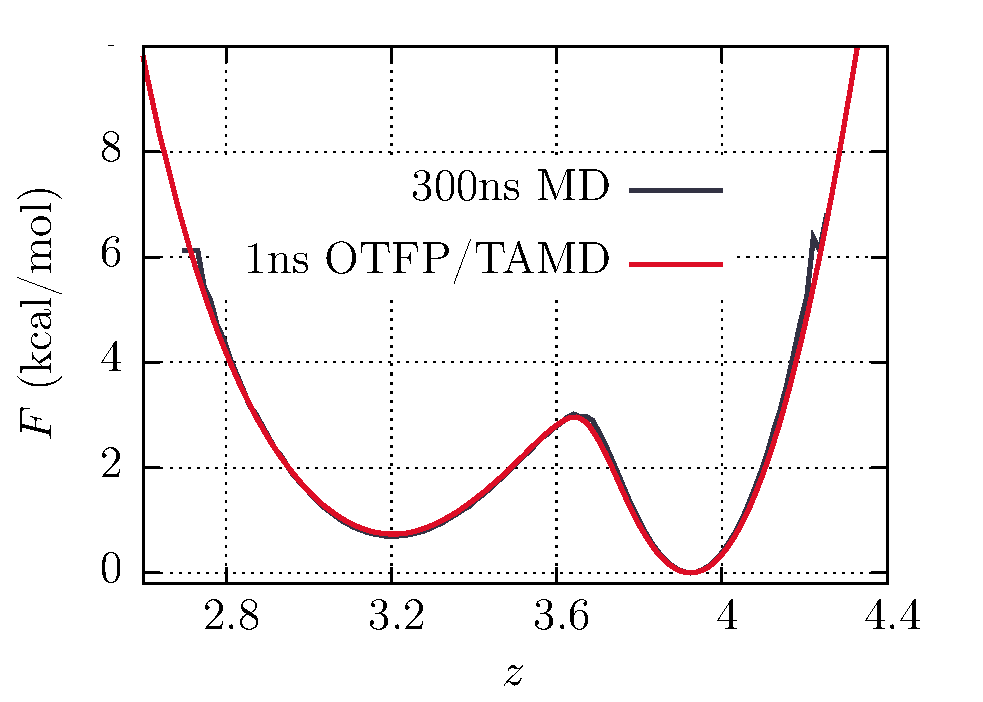
\includegraphics[width=0.45\textwidth]{otfpc4}
            }
            ++(0,0) node(config)[graphics,anchor=south east]{
                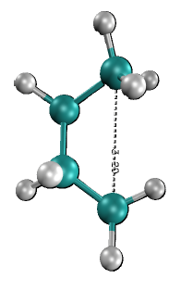
\includegraphics[width=0.16\textwidth]{butane}
            };
        \end{tikzpicture}
\end{frame}



% %\begin{frame}[fragile]{DAVEI: Dual-Acting Virolytic Entry Inhibitors}
\begin{tikzpicture}[scaleall=1.0]
\pcuad{\textwidth}{\textheight}
%\showcuad
\path(nw) ++(-0.75,0.15) node(text)[anchor=north west,text 
width=1.1\textwidth]{{\tiny \textcolor{red!80!black}{Contarino, Bastian, Sundaram, McFadden, Duffy, Gangupomu, Baker, Abrams, Chaiken, {\it Antimicrob.
 Agents Chemother.} 2013, {\bf 57}:4743\\*[-1em]
Parajuli, Acharya, Yu, Ngo, Rashad, Abrams, Chaiken, {\it Biochemistry} 2016 {\bf 55}:6100}}};
\path(nw) ++(-1,-1) node(text2)[anchor=north west,text width=1.1\textwidth]{
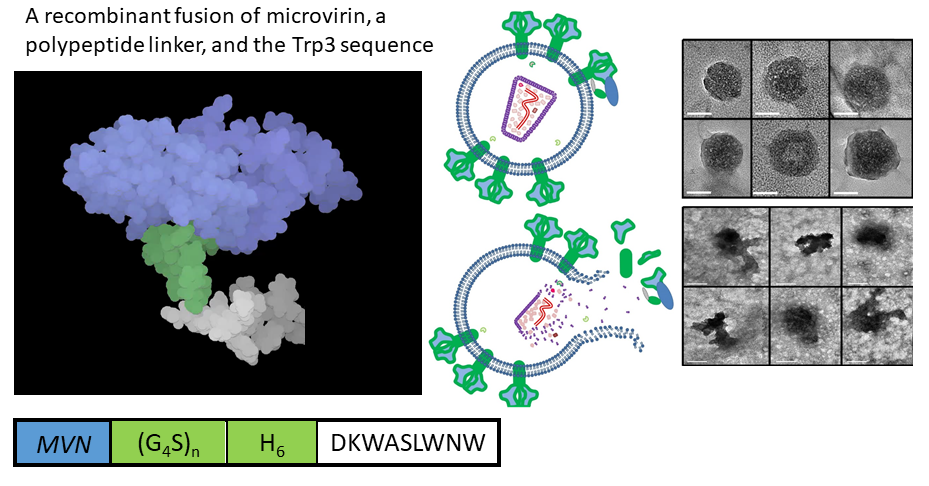
\includegraphics[width=\textwidth]{davei_whatisit.png}};
\end{tikzpicture}
\end{frame}


% %% asparagines: 262 dash
% 332 dot
% 386 dash dot-dot
% 392 long-dash dot
% 448 solid
\begin{frame}[fragile]{OTFP Predicts DAVEI Activity Dependence on Linker Length}
\begin{tikzpicture}[scaleall=1.0]
\pcuad{\textwidth}{\textheight}
%\showcuad
\path(nw) ++(-0.75,0.15) node(text)[anchor=north west,text 
width=\textwidth]{{\tiny \textcolor{red!80!black}{S. Gossert and CFA, {\it Protein Science}, vol. 29, pp. 2304-2310, 2020. doi:10.1002/pro.3949}}};
\path(nw) ++(-0.75,-4) node(text2)[anchor=north west,text width=0.5\textwidth]{
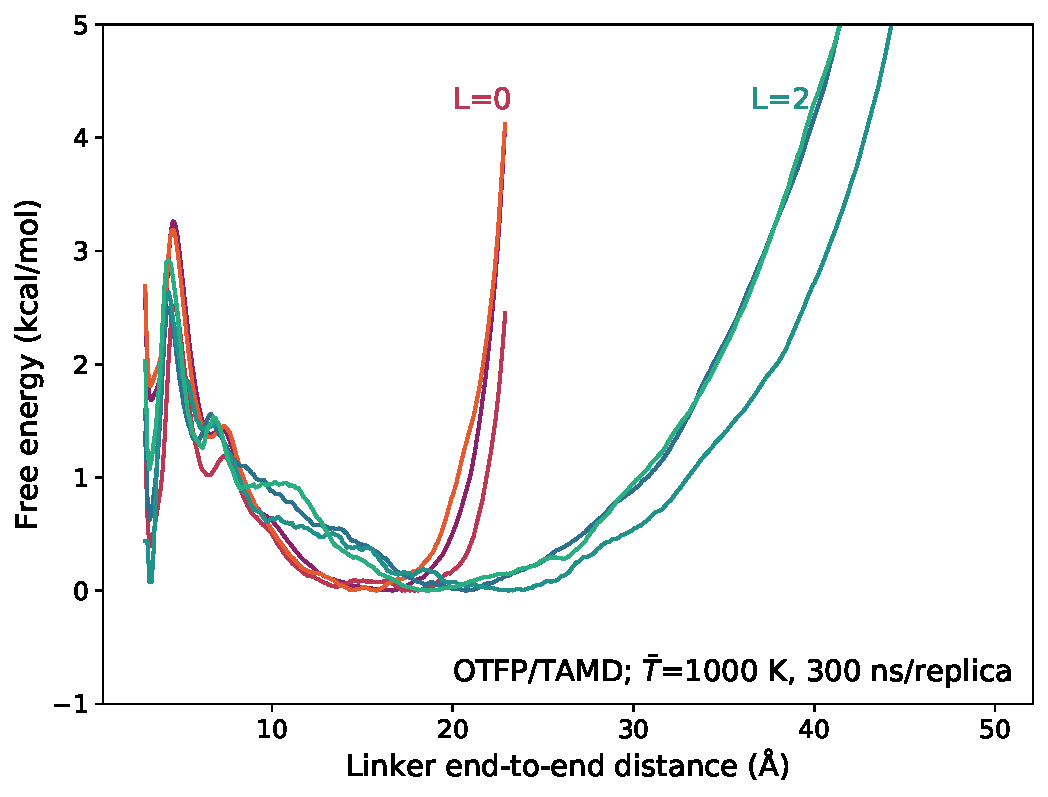
\includegraphics[width=\textwidth]{linker_pmf.pdf}};
\path(nw) ++(0.5,-0.15) node(text2)[anchor=north west,text width=0.4\textwidth]{
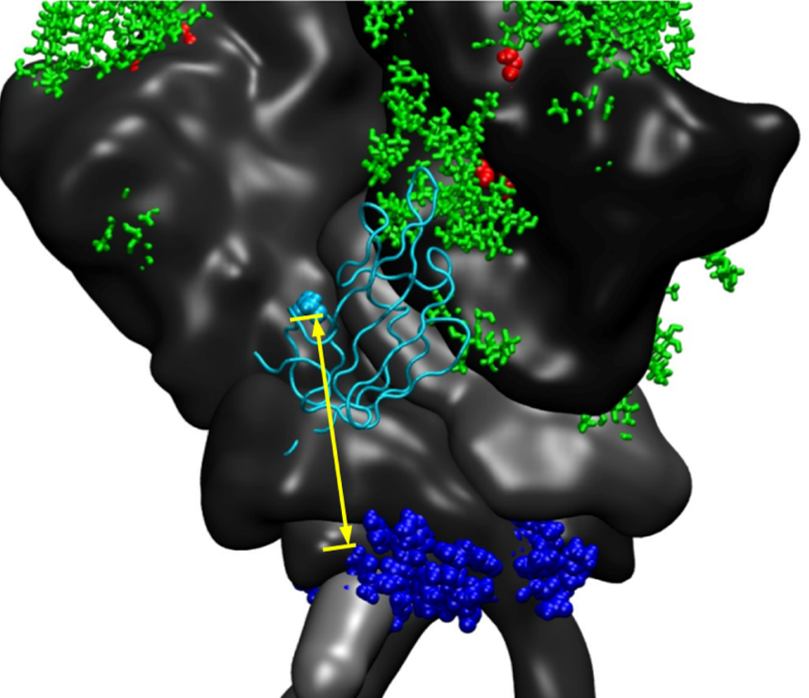
\includegraphics[width=\textwidth]{env+mvn_dist.png}};
\path(nw) ++(5,0) node(text2)[anchor=north west,text width=0.6\textwidth]{
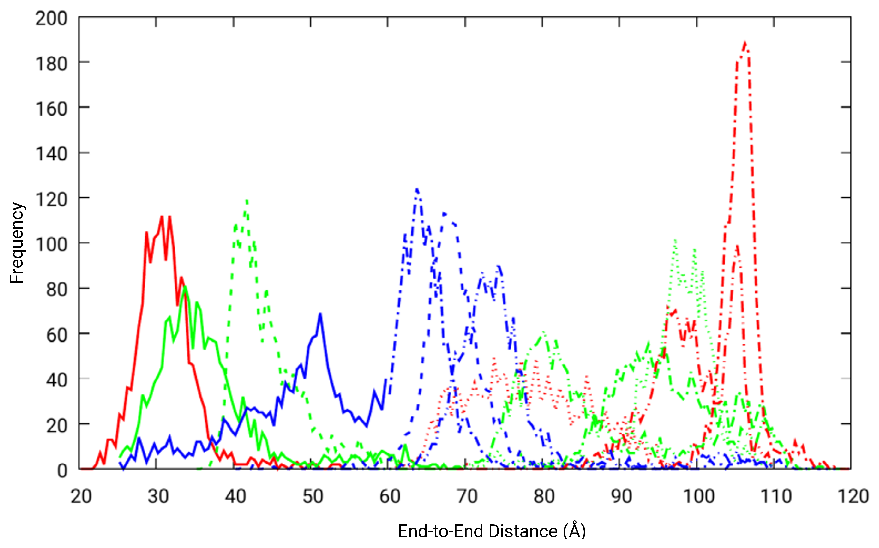
\includegraphics[width=\textwidth]{davei_env_mvn_dist_hist_1.png}};
\path(nw) ++(5.75,-0.25) node(text3)[anchor=north west,text width=0.5\textwidth]{\tiny MD, 40 ns};
\path(nw) ++(5.5,-4.25) node(text2)[anchor=north west,text width=0.45\textwidth]{
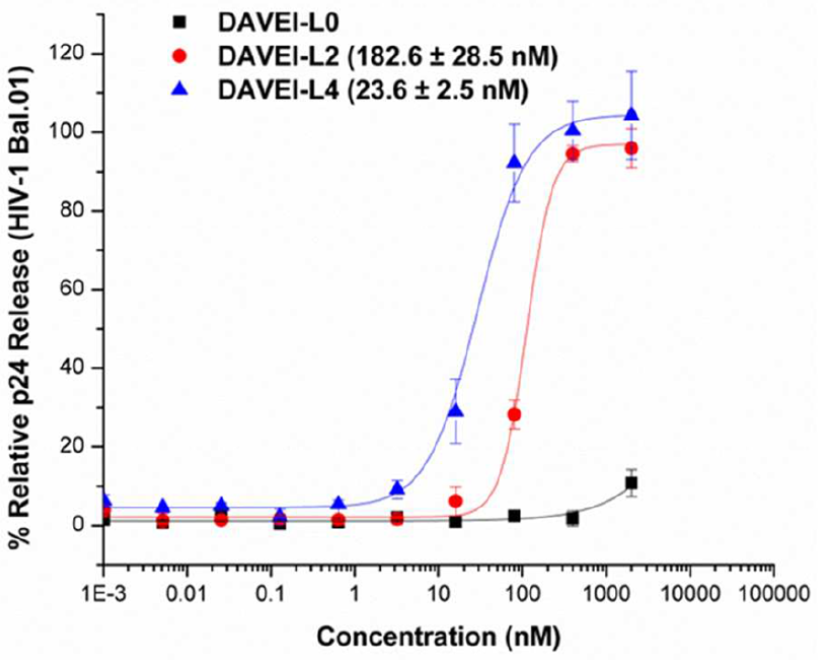
\includegraphics[width=\textwidth]{DAVEI-L02-experiment.png}};
\path(nw) ++(6.5,-0.5) node(text2)[anchor=north west,text width=0.1\textwidth]{
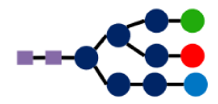
\includegraphics[width=\textwidth]{man9.png}};
\path(nw) ++(8.5,-0.4) node(text2)[anchor=north west,text width=0.08\textwidth]{
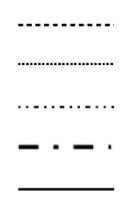
\includegraphics[width=\textwidth]{dashkey.png}};
\path(nw) ++(8.5,-0.25) node(text3)[anchor=north west,text width=0.5\textwidth]
{\tiny N-linked glycans};
\path(nw) ++(8.5,-0.4) node(text3)[anchor=north west,text width=0.5\textwidth]
{\tiny 262};
\path(nw) ++(8.5,-0.66) node(text3)[anchor=north west,text width=0.5\textwidth]
{\tiny 332};
\path(nw) ++(8.5,-0.92) node(text3)[anchor=north west,text width=0.5\textwidth]
{\tiny 386};
\path(nw) ++(8.5,-1.18) node(text3)[anchor=north west,text width=0.5\textwidth]
{\tiny 392};
\path(nw) ++(8.5,-1.48) node(text3)[anchor=north west,text width=0.5\textwidth]
{\tiny 448};
\path(nw) ++(-0.75,-1.5) node(label1)[anchor=north west,text width=0.4\textwidth]{MVN at\\N448 glycan};
\path(nw) ++(0.6,-2.4) node(label2)[anchor=north west,text width=0.2\textwidth]{40 \AA};
\path(nw) ++(-0.2,-3.2) node(label3)[anchor=north west,text width=0.4\textwidth]{Trp3 at MPER};
\end{tikzpicture}
\end{frame}



\begin{frame}[fragile]{Potassium Channels}
\begin{tikzpicture}[scaleall=1.0]
\pcuad{\textwidth}{\textheight}
%\showcuad
\path(nw) ++(-0.5,0.25) node(corner)[graphics,anchor=north 
west]{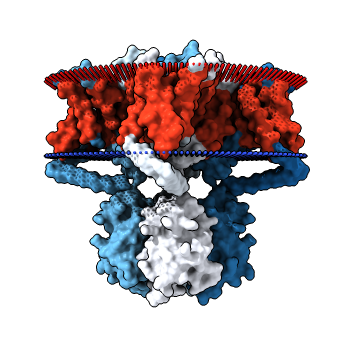
\includegraphics[width=0.33\textwidth]{2a79.png}};
\path(wp) ++(-0.0,1.0) node(corner)[graphics,anchor=north 
west]{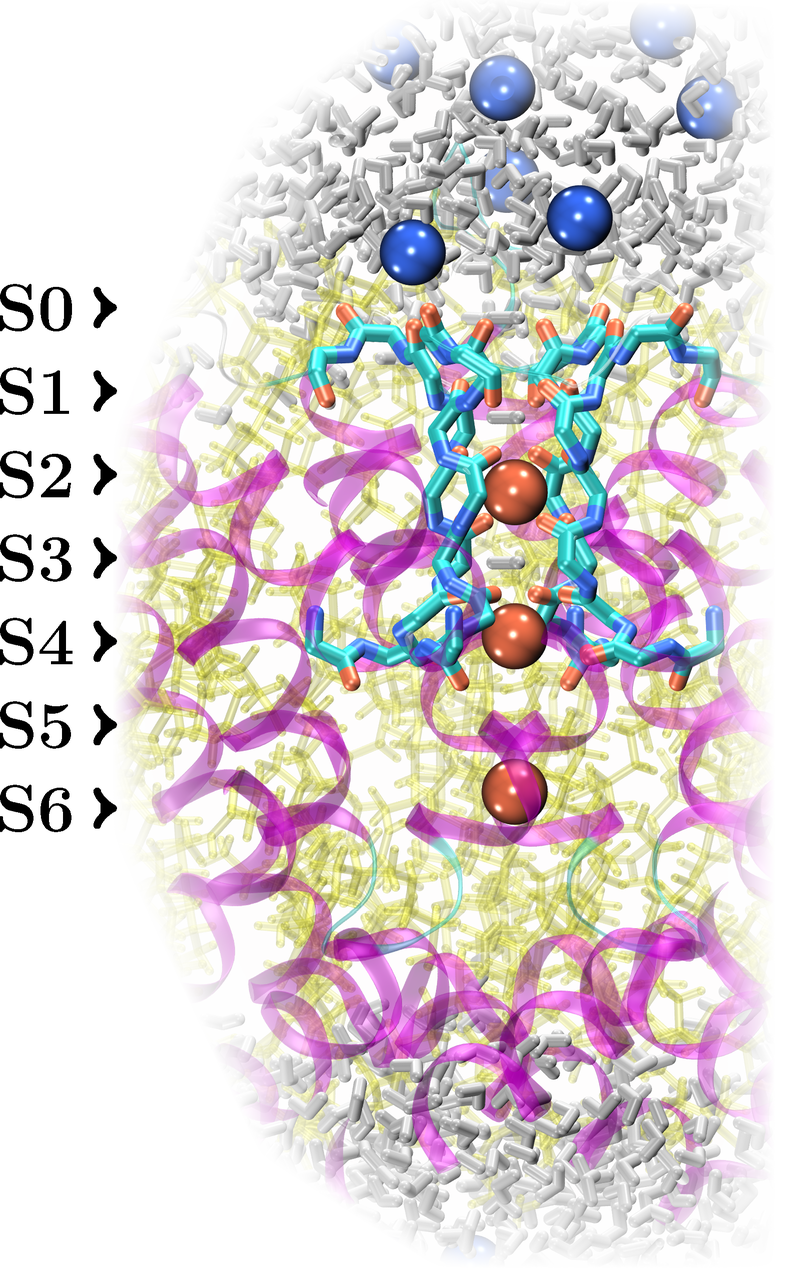
\includegraphics[width=0.25\textwidth]{Kv12_sfilter.png}};
\path(nw) ++(3,0) node(text)[anchor=north west,text width=0.75\textwidth]{
\begin{itemize}
\item Responsible for cell membrane {\em depolarization} in action-potential firing
\item Malfunctions: ``channelopathies'' like episodic ataxia, neuromyotonia, seizure, and tinnitus
\item Selectivity mechanism is not well-understood because the selectivity filter is complicated
\end{itemize}
};
\path(wp) ++(3.5,0.0) node(plot)[graphics,anchor=north west]{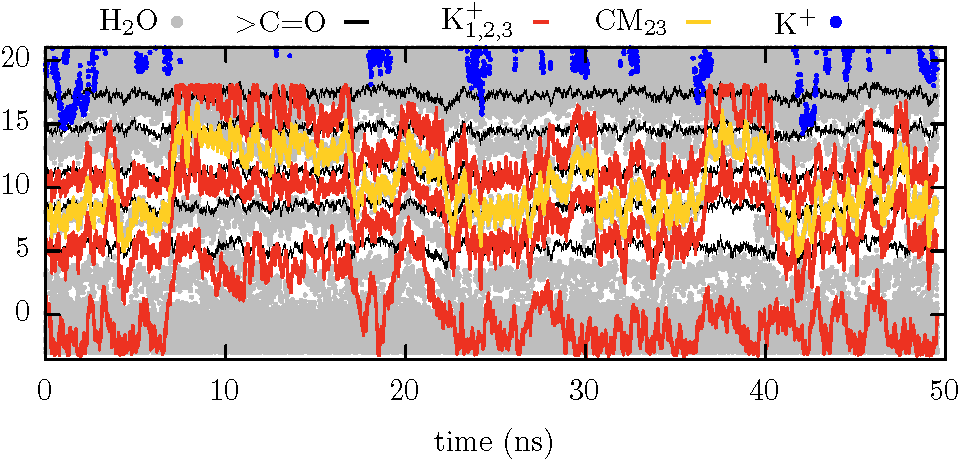
\includegraphics[width=0.65\textwidth]{fullions-crop.png}};
\path(nw) +(0,0.2) node(cite)[anchor=north west]{\tiny \textcolor{red!80!black}{S. A. Paz, L. Maragliano, and CFA {\em J. Chem. Theory. Comput.} {\bf 14}:2743-2750 (2018)}};
\end{tikzpicture}

\end{frame}



\begin{frame}{2D OTFP: Transport Minimum Free-Energy Pathways}
\begin{tikzpicture}
\pcuad{\textwidth}{\textheight}
%\showcuad
\path(nw) +(0,0.2) node(cite)[anchor=north west]{\tiny \textcolor{red!80!black}{S. A. Paz, L. Maragliano, and CFA {\em J. Chem. Theory. Comput.} {\bf 14}:2743-2750 (2018)}};
\path(nw) +(0,0) node(image)[anchor=north west]{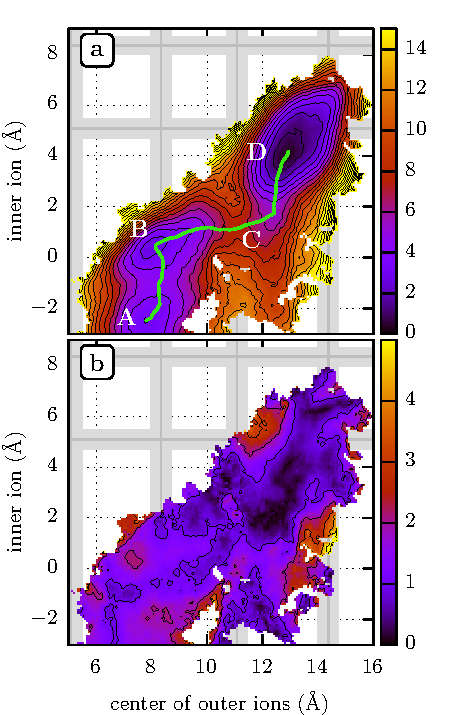
\includegraphics[width=0.5\textwidth]{fullfes_path_err.pdf}};
\path(nw) +(1.5,-4) node(errlab)[anchor=north west]{Error, $N$=3};
\path(nw) +(5,-1.5) node(bullets)[anchor=north west,text width=0.5\textwidth]{\begin{itemize}
\item A$\rightarrow$B: Innermost ion moves up one position
\item B$\rightarrow$C: CM$_{2,3}$ moves up one position, followed quickly by
\item C$\rightarrow$D: Innermost ion moves up one more position
\item $\Rightarrow$ Net translocation of one K$^+$
\item What role is water playing?
\end{itemize}};
\end{tikzpicture}
\end{frame}



\begin{frame}{Water Restraints: Ion-Tethered vs. Excluded-from-Filter}
\begin{tikzpicture}
\pcuad{\textwidth}{\textheight}
%\showcuad
\path(nw) +(0,0) node(image)[anchor=north west]{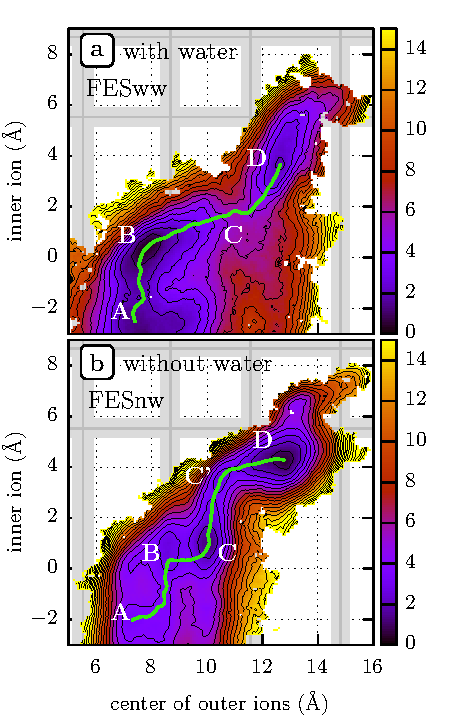
\includegraphics[width=0.5\textwidth]{wc_fes.pdf}};
\path(nw) +(5,-1.5) node(bullets)[anchor=north west,text width=0.5\textwidth]{\begin{itemize}
\item With one water tethered to each K$^+$, FES resembles unrestrained one
\item With water excluded from channel, ion motion is less concerted, more ``hard-knock'' like
\end{itemize}};
\end{tikzpicture}
\end{frame}



\begin{frame}{Free-Energy Profiles along MFEP's}
\begin{tikzpicture}
\pcuad{\textwidth}{\textheight}
%\showcuad
\path(nw) +(0,0.2) node(cite)[anchor=north west]{\tiny \textcolor{red!80!black}{S. A. Paz, L. Maragliano, and CFA {\em J. Chem. Theory. Comput.} {\bf 14}:2743-2750 (2018)}};
\path(np) +(0,0) node(image)[anchor=north]{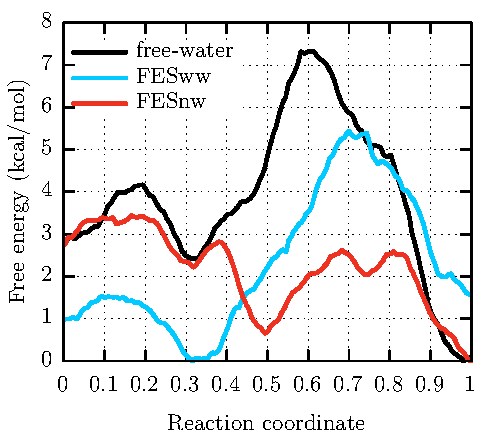
\includegraphics[width=0.67\textwidth]{paths.pdf}};
\path(nw) +(0,-6) node(bullets)[anchor=north west,text width=\textwidth]{\begin{itemize}
\item Energy barriers for unrestricted and ion-tethered water systems are similar; suggests intercalated water is preferred
\item Dry filter shows shallower barriers; dry transport might be faster if water could be actively excluded
\end{itemize}};
\end{tikzpicture}
\end{frame}



% %\section{The String Method}

% %\input{frame_string_method}

% \section{Markovian Milestoning}

% \begin{frame}[fragile]{Building Up Markovian Milestoning Calculations of Kinetics}
\begin{tikzpicture}[scaleall=1.0]
\pcuad{\textwidth}{\textheight}
%\showcuad
\path(nw) ++(-0.75,0.15) node(text)[anchor=north west,text 
width=\textwidth]{{\tiny \textcolor{red!80!black}{T.-Q. Yu, M. Lapelosa, E. Vanden-Eijnden, and \underline{CFA}
{\em JACS} {\bf 137}:3041 (2015)}}};
\path(nw) ++(-0.5,-1.0) node(moretext)[anchor=north west,text width=0.5\textwidth]{
\begin{itemize}
\item Free energy and minimum free-energy pathways (MFEPs) as functions of ligand location via \textcolor{red}{single-sweep reconstruction}
\item Site-to-site and site-to-portal mean first-passage times (MFPT's) for O$_{\sf 2}$ diffusion along MFEP's using \textcolor{green!80!black}{Markovian milestoning}
\end{itemize}};
\path(nw) ++(6,-1) node(image)[anchor=north west]{
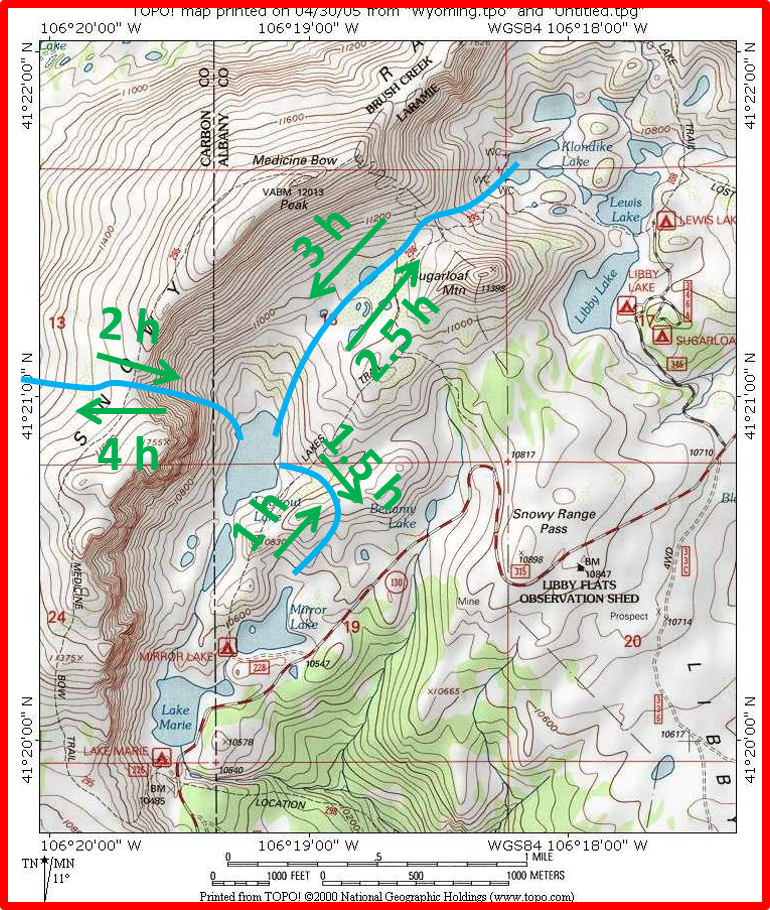
\includegraphics[width=0.5\textwidth]{topo_medicine_bow}};
\end{tikzpicture}
\end{frame}


% \begin{frame}[fragile]{Single-Sweep Free-Energy Reconstruction}
\begin{tikzpicture}[scaleall=1.0]
\pcuad{\textwidth}{\textheight}
%\showcuad
\path(nw) ++(-0.75,0.15) node(cites)[anchor=north west,text 
width=\textwidth]{{\tiny \textcolor{red!80!black}{
L. Maragliano and E. Vanden-Eijnden, {\it J Chem Phys} {\bf 88}:184110 (2008)
}}};
\path(nw) +(0.0,-1.0) node(text1) [anchor=north west,text width=\textwidth] {
At each $\zb_i$, use \textcolor{green!80!black}{restrained MD} to estimate mean forces $\fb_i$:
\begin{displaymath}
\fb_i = -\left.\frac{\partial F}{\partial \zb}\right|_{\zb_i} \approx \langle \kappa\left[\thetab(\xb)-\zb\right]\rangle_{\zb_i}.
\end{displaymath}
Cast free energy $F(\zb)$ as a superposition of radial Gaussian basis functions $\phi_i$:
\begin{displaymath}
\tilde{F}(\zb) = \sum_i a_i \phi_i (|\zb-\zb_i|;\sigma)
\end{displaymath}
Determine $\tilde{F}$ by finding $\ab,\sigma$ to minimize an error $E(\ab,\sigma)$:
\begin{displaymath}
E(\ab,\sigma) = \sum_i\left|\sum_{i^\prime} a_{i^\prime} \nabla_{\zb}\phi(|\zb_i-\zb_{i^\prime}|;\sigma)+\fb_i\right|^2
\end{displaymath}
};
\end{tikzpicture}
\end{frame}


% \begin{frame}[fragile]{Milestoning: Temporal Coarse-Graining of MD}
\begin{tikzpicture}[scaleall=1.0]
\pcuad{\textwidth}{\textheight}
%\showcuad
\path(nw) +(-0.75,0.15) node(text)[anchor=north west,text 
width=\textwidth]{{\tiny \textcolor{red!80!black}{A. K. Faradjian and R. Elber {\it J Chem Phys} {\bf 120}:010880 (2004).}}};
\path(nw) +(-0.75,-0.5) node(text1)[anchor=north west,text width=0.5\textwidth]{
Coarsening of a hypothetical infinitely long MD trajectory onto a \textcolor{red}{jump process}};
\path(nw) +(-0.75,-2) node(image1)[anchor=north west]{
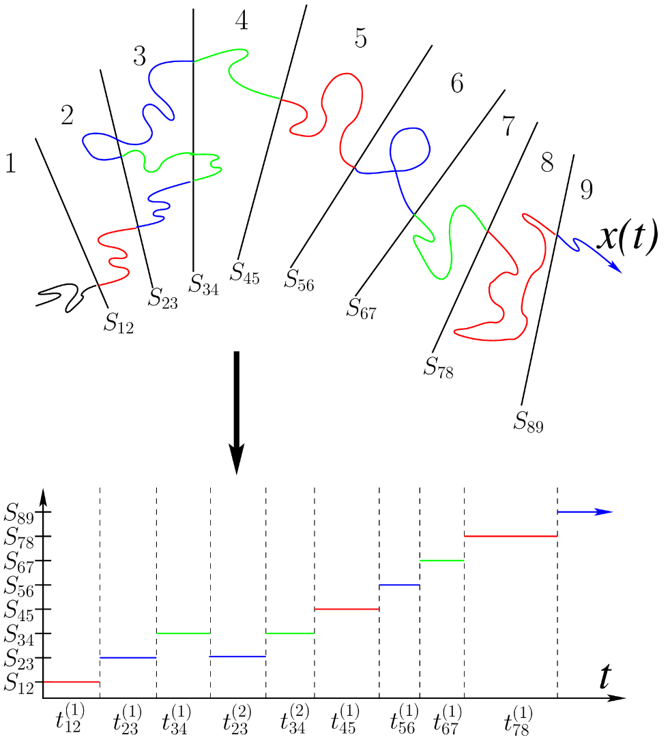
\includegraphics[width=0.5\textwidth]{milestoning1}};
\path(nw) +(5,0) node(text2) [anchor=north west,text width=0.5\textwidth]{
\begin{center}
Coarse-grained kinetics are fully described by a \textcolor{blue}{rate matrix}:
\end{center}
\begin{displaymath}
q_{ik,ij} = \left\{\begin{array}{ll}
\frac{\ds N_{ik,ij}}{\ds R_{ij}} & \mbox{if}\ R_{ij}>0;\\
0 & \mbox{if}\ R_{ij}=0,
\end{array}\right.
\end{displaymath}
where
\begin{align*}
N_{ik,ij} =& \left\{\begin{array}{l}
\mbox{\# of times trajectory}\\
\mbox{collides with $S_{ik}$ after}\\
\mbox{last hitting $S_{ij}$}
\end{array}\right\},\\
R_{ij} = &\left\{\begin{array}{l}
\mbox{total amount of time for}\\
\mbox{which $S_{ij}$ was the last}\\
\mbox{milestone hit}
\end{array}\right\},\\
& = \sum_m t_{ij}^{(m)}.
\end{align*}
};
\end{tikzpicture}
\end{frame}


% \begin{frame}[fragile]{Making Milestoning Practical: Transition-Path Theory and \\ Markovian Milestoning in Voronoi Tesselations}
\begin{tikzpicture}[scaleall=1.0]
\pcuad{\textwidth}{\textheight}
%\showcuad
\path(nw) ++(-0.75,0.15) node(text)[anchor=north west,text 
width=\textwidth]{{\tiny \textcolor{red!80!black}{
E. Vanden-Eijnden et al. {\it J Chem Phys} {\bf 130}:194101 (2009).}}};
\path(nw) ++(-0.75,-0.5) node(text2)[anchor=north west,text width=1.1\textwidth]{
Estimate \textcolor{blue}{$\ds q_{ik,ij}$} using MD confined to Voronoi cells in feature-space};
\path(nw) ++(-0.75,-1.5) node(image1)[anchor=north west]{
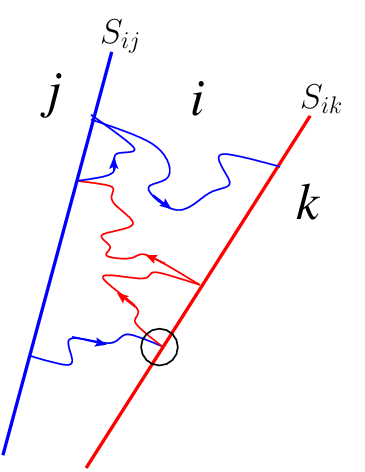
\includegraphics[width=0.4\textwidth]{milestoning2}};
\path(nw) ++(4.25,-1.0) node(text3)[scale=0.7,anchor=north west,text width=0.8\textwidth]{
In each cell $i$, use confined MD of duration $T_i$ to tally:
\begin{enumerate}
\item $N^i_{ik,ij}$,
\item $R^i_{ij}$,\ and,
\item $N^i_{i\rightarrow j}$: \# of transition attemps from $i$ to any neighbor $j$.
\end{enumerate}
Compute apparent transition rate constants:
\begin{displaymath}
k_{i\rightarrow j} = \frac{\ds N^i_{i\rightarrow j}}{\ds T_i}
\end{displaymath}
And enforce equilibrium among all $\Lambda$ cells, so
\begin{displaymath}
\sum_{j=1,j\ne i}^{\Lambda} \pi_j k_{j\rightarrow i} = \pi_i\sum_{j=1;j\ne i}^{\Lambda} k_{i\rightarrow j}\ \ \sum_i\pi_i = 1
\end{displaymath}
providing equilibrium probabilities to be in cell $i$, $\pi_i$.  This allows construction of $q_{ik,ij}$:
\begin{displaymath}
q_{ik,ij} = \frac{\ds \pi_i N^i_{ik,ij}/T_i}{\ds \pi_i R^i_{ij}/T_i + \pi_j R_{ij}^j/T_j}.
\end{displaymath}
};
\end{tikzpicture}
\end{frame}



% \begin{frame}[fragile]{MSOX:  A Prototypical Flavoenzyme}
\begin{tikzpicture}[scaleall=1.0]
\pcuad{\textwidth}{\textheight}
%\showcuad
\path (nw) ++(0,0) node (heading) [anchor=north west,text width=\textwidth] 
{MSOX is a bacterial enzyme that uses the \textcolor{orange!80!black}{flavin} redox cycle to catalyze oxidative demethylation of sarcosine to glycine.};
\path(c2) ++(0,0.5) node (FoSr) [shape=rectangle,draw] {F$_{\sf O}$S$_{\sf R}$}
          ++(-2,-1.5) node (Fo) [shape=rectangle,draw] {F$_{\sf O}$}
          ++(+2,-1.5) node (Fr) [shape=rectangle,draw] {F$_{\sf R}$}
          ++(+2,1.5) node (FrPo) [shape=rectangle,draw] {F$_{\sf R}$P$_{\sf O}$}
          ++(-2,-3.5) node (FrPoO2) [shape=rectangle,draw] {F$_{\sf R}$P$_{\sf O}$O$_{\sf 2}$};
\path(Fo)  +(0.5,1) node (Sr) [shape=rectangle] {S$_{\sf R}$};
\path(FrPo) +(-1.5,0.0) node (Poa) [shape=rectangle] {P$_{\sf O}$};
\path(FrPo) +(0.0,-2) node (O2a) [shape=rectangle] {O$_{\sf 2}$};
\path(O2a) +(-2.75,0.0) node (O2b) [shape=rectangle] {O$_{\sf 2}$};
\path(Fo) +(1.5,0) node (H2O2a) [shape=rectangle] {H$_{\sf 2}$O$_{\sf 2}$};
\path(Fo) +(-0.5,-1.5) node (Pob) [shape=rectangle] {P$_{\sf O}$};
\path(Pob) +(0,-1) node (H2O2b) [shape=rectangle] {H$_{\sf 2}$O$_{\sf 2}$};
\draw [->,thick] (Fo.north east) -- (FoSr.south west) node(attractor1)[pos=0.90]{};
\draw [->,thick,snake] (FoSr.south east) -- (FrPo);
\draw [->,thick] (FrPo.south west) -- (Fr.north east) node(attractor2)[pos=0.10]{};
\draw [->,thick] (Fr.north west) -- (Fo.south east) node (attractor5)[pos=0.10]{} node(attractor4)[pos=0.70]{};
\draw [->,thick] (FrPo.south) -- (FrPoO2.north east) node(attractor3)[pos=0.60]{};
\draw [->,thick] (FrPoO2.north west) -- (Fo.south) node(attractor6)[pos=0.2]{} node(attractor7)[pos=0.6]{};
\draw [<-,thick] (FoSr.south west) .. controls (attractor1.south west) .. (Sr.east);
\draw [->,thick] (FrPo.south west) .. controls (attractor2.south west) .. (Poa.south east);
\draw [<-,thick,color=red] (FrPoO2.north east) .. controls (attractor3.south) .. (O2a.west);
\draw [->,thick] (Fr.north west) .. controls (attractor4.north west) .. (H2O2a.south west);
\draw [<-,thick,color=blue] (Fo.south east) .. controls (attractor5.north west) .. (O2b.north);
\draw [->,thick] (FrPoO2.north west) .. controls (attractor6.north west) .. (H2O2b.east);
\draw [->,thick] (FrPoO2.north west) .. controls (attractor7.north west) .. (Pob.east);
\path(nw) +(6,-1) node (image) [graphics,anchor=north west] {
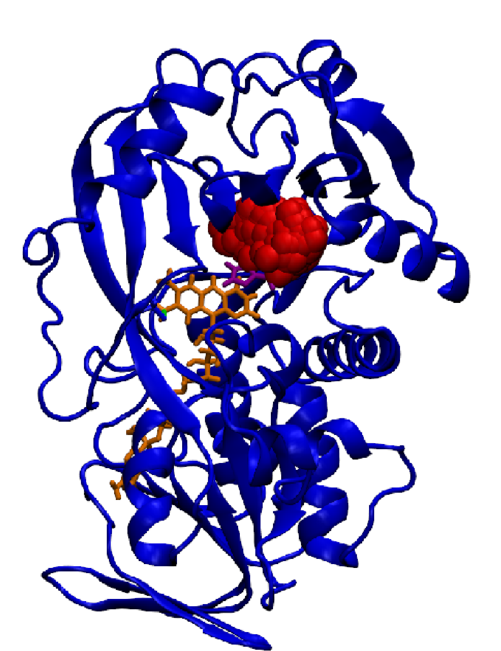
\includegraphics[width=0.45\textwidth]{msox_o2_1}};
\path(c3) +(-2,-0.5) node (sometext) [shape=rectangle,anchor=north west,text width=\textwidth] {
\textcolor{blue}{Ping-pong} vs. \textcolor{red}{Modified ping-pong}};
\end{tikzpicture}
\end{frame}


% \begin{frame}[fragile]{Experimental Support for Modified Ping-Pong}
\begin{tikzpicture}[scaleall=1.0]
\pcuad{\textwidth}{\textheight}
%\showcuad
\path(nw) ++(-0.25,-0.4) node(plot)[graphics,anchor=north west]{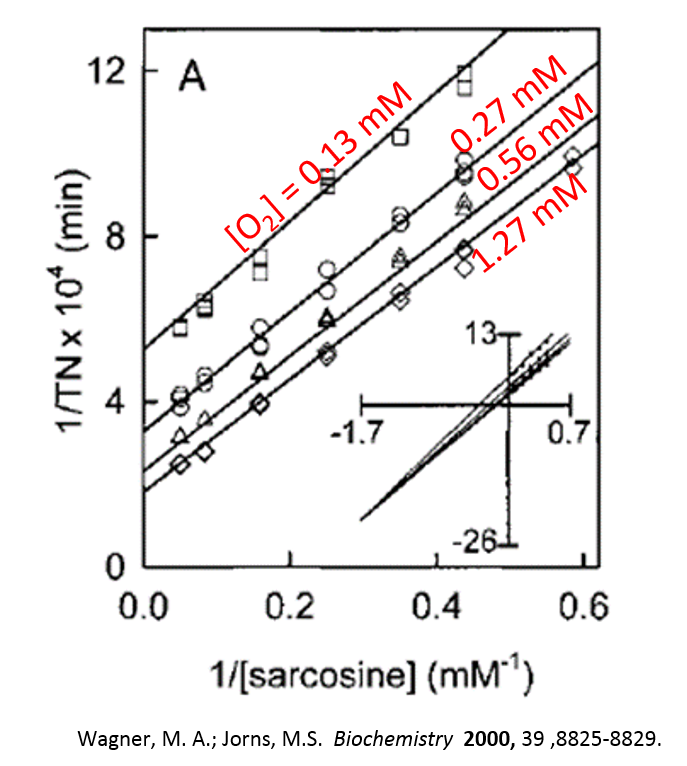
\includegraphics[width=0.6\textwidth]{msox_jorns_expt}}
          ++(6.5,-0.0) node(text) [shape=rectangle,anchor=north west,text width=0.4\textwidth] {
          Lineweaver-Burk slope-dependence on [O$_{\sf 2}$] indicates [O$_{\sf 2}$] and [S$_{\sf R}$] are not independent, suggesting \textcolor{red}{MPP}.}
          ++(0.0,-3.0) node(moretext) [shape=rectangle,anchor=north west,text width=0.4\textwidth]{
          \textcolor{green!80!black}{\bf Hypothesis:} MPP implies kinetics of O$_{\sf 2}$ entry and exit should be 
          sensitive to whether or not substrate is bound.  Test using simulations!};

\end{tikzpicture}
\end{frame}


% \begin{frame}[fragile]{Three-Dimensional Free-Energy $F(\zb)$ for O$_{\sf 2}$ in MSOX}
\begin{tikzpicture}[scaleall=1.0]
\pcuad{\textwidth}{\textheight}
%\showcuad
\path(nw) ++(-0.75,0.15) node(cites)[anchor=north west,text 
width=\textwidth]{{\tiny \textcolor{red!80!black}{
A. Bucci and \underline{CFA}, {\it J Chem Theory Comput} {\bf 10}:2668 (2014)
}}};
\path(nw) +(-1,-1) node (image1) [graphics,anchor=north west] {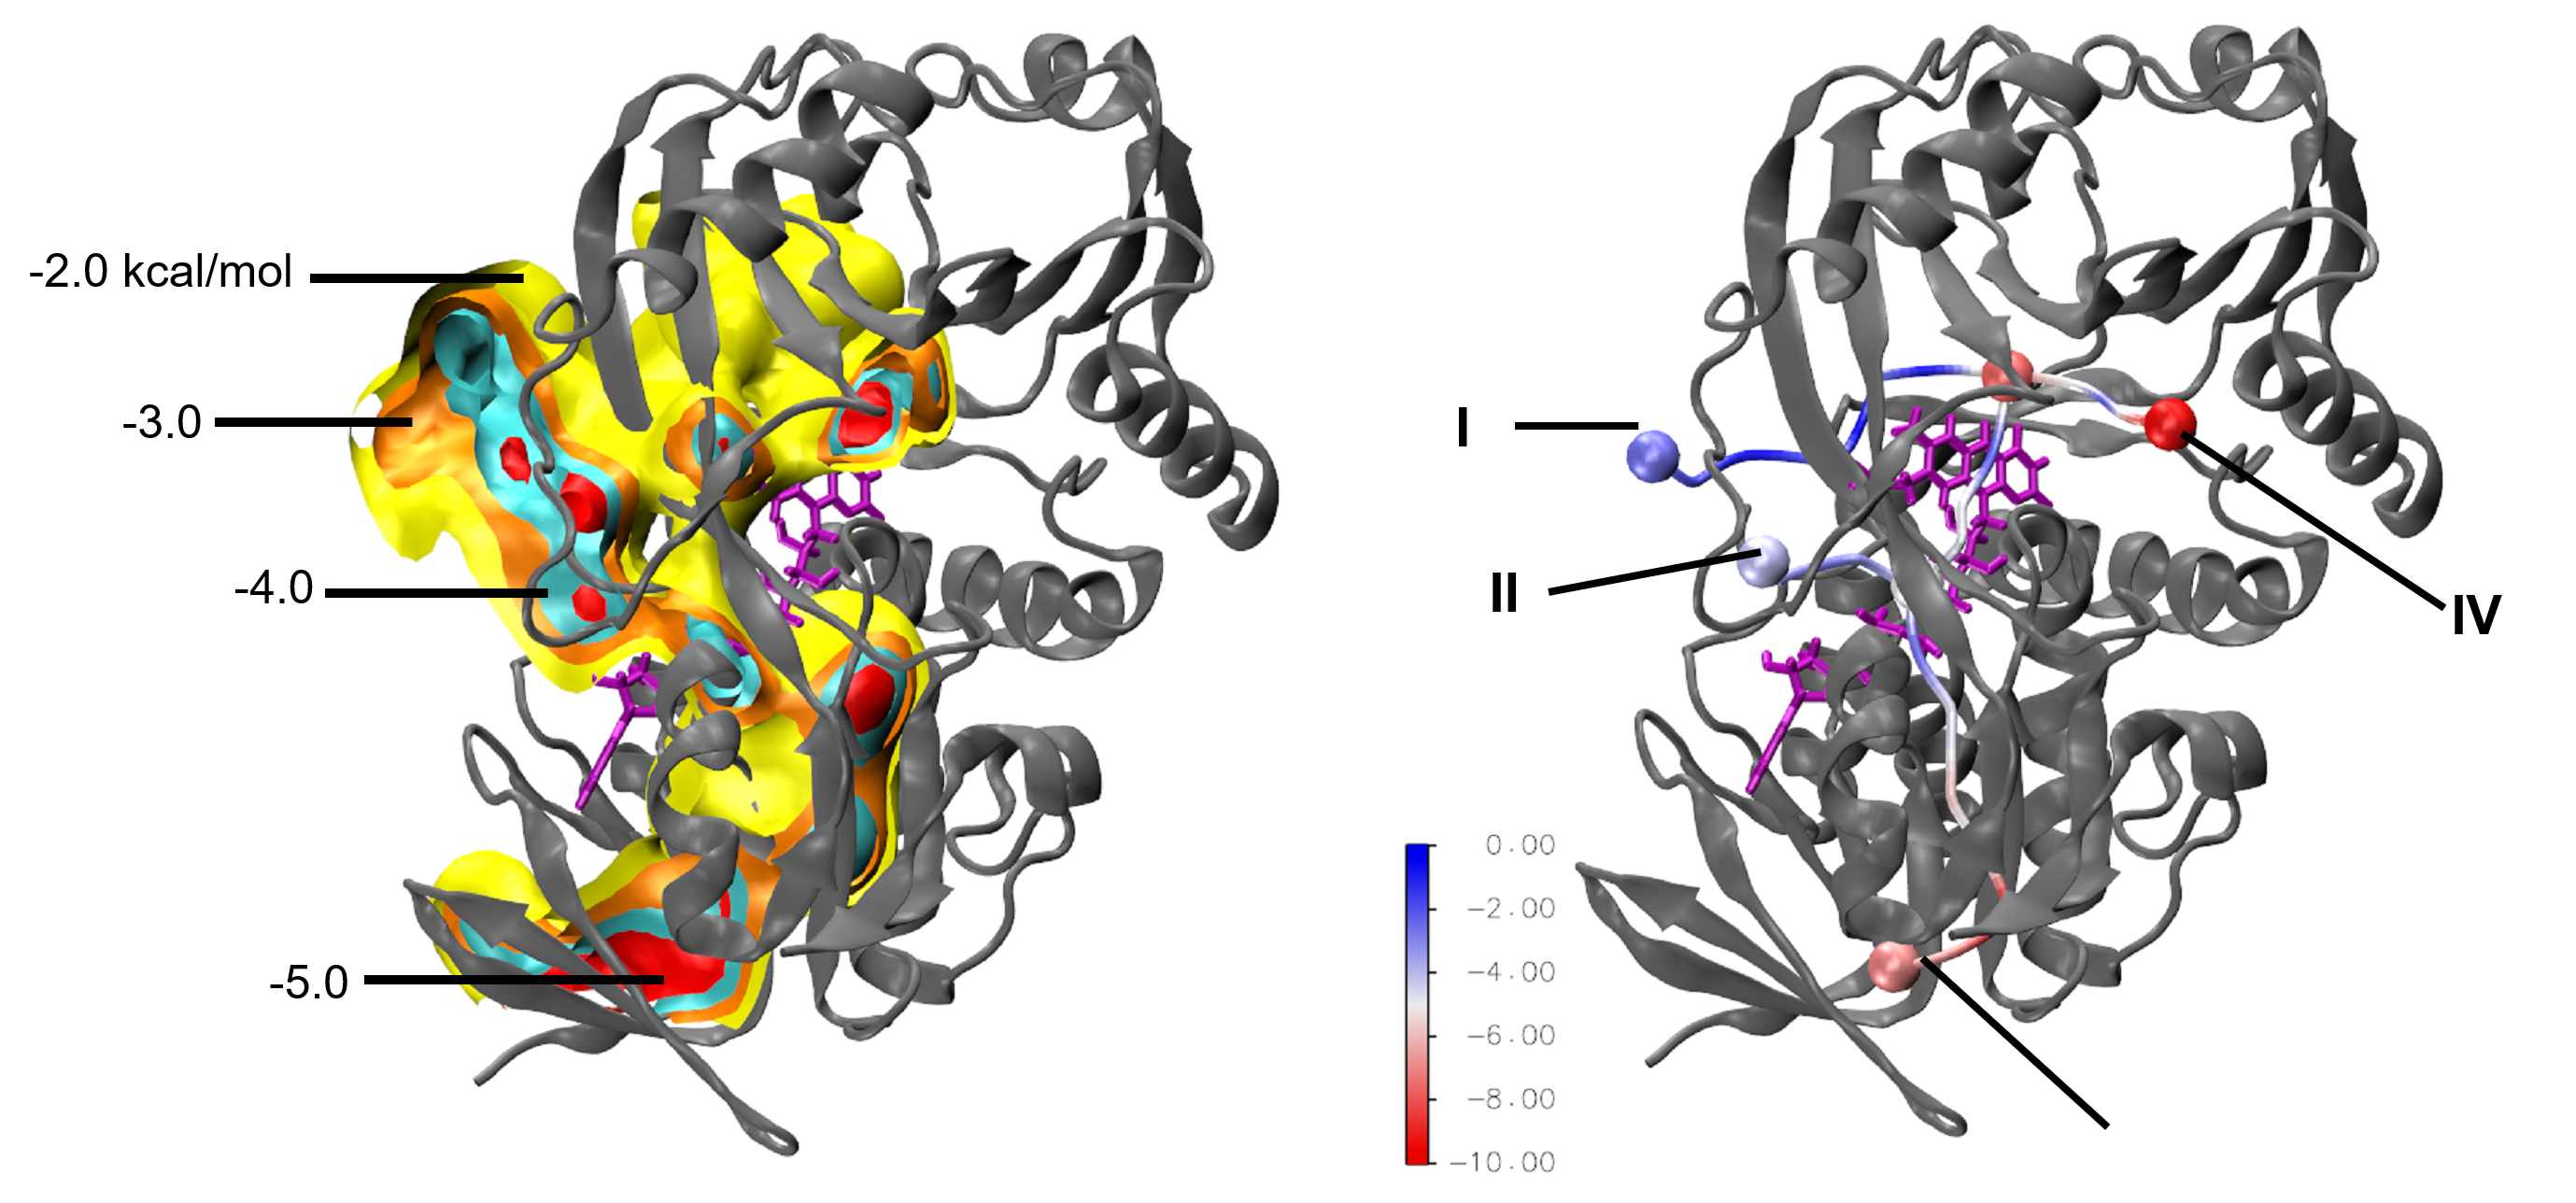
\includegraphics[width=1.2\textwidth]{msox_fep_sites.png}};
\end{tikzpicture}
\end{frame}



% \begin{frame}[fragile]{Hitting Points on Milestones along O$_{\sf 2}$-Diffusion Pathways in MSOX}
\begin{tikzpicture}[scaleall=1.0]
\pcuad{\textwidth}{\textheight}
%\showcuad
\path(nw) ++(-0.75,0.15) node(text)[anchor=north west,text 
width=\textwidth]{{\tiny \textcolor{red!80!black}{
A. Bucci, T.-Q. Yu, E. Vanden-Eijnden and \underline{CFA} {\it J Chem Theory Comput} {\bf 12}:2964 (2016).}}};
\path(nw) ++(2.5,-0.5) node(image1)[anchor=north west]{
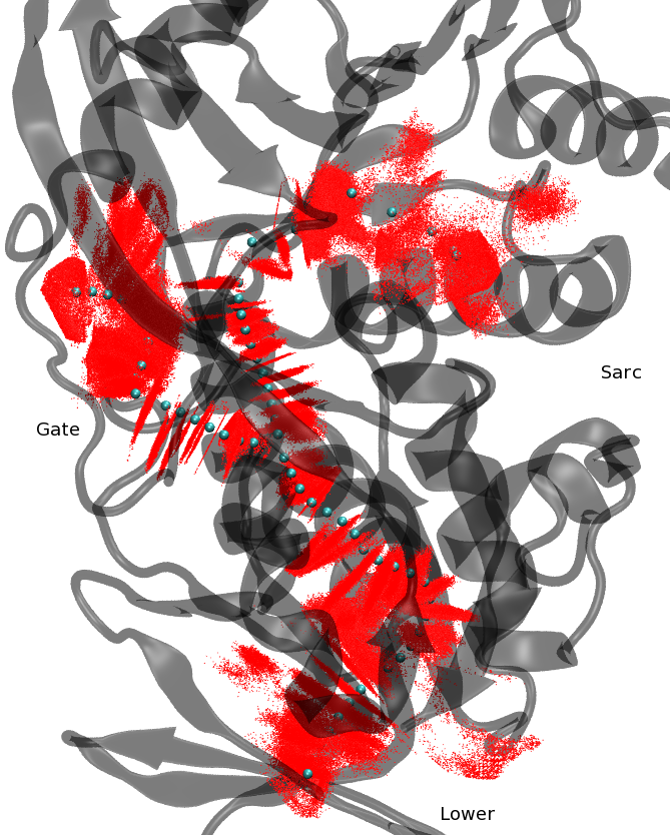
\includegraphics[width=0.5\textwidth]{msox_milestoning}};
\end{tikzpicture}
\end{frame}


% \begin{frame}[fragile]{Milestoning Predicts O$_{\sf 2}$ Kinetics Are Sensitive to Substrate}
\begin{tikzpicture}[scaleall=1.0]
\pcuad{\textwidth}{\textheight}
%\showcuad
\path(nw) ++(-0.75,0.15) node(text)[anchor=north west,text 
width=\textwidth]{{\tiny \textcolor{red!80!black}{
A. Bucci, T.-Q. Yu, E. Vanden-Eijnden and \underline{CFA} {\it J Chem Theory Comput} {\bf 12}:2964 (2016).}}};
\path(nw) ++(-0.25,0.5) node(table)
[shape=rectangle,anchor=north west,text width=\textwidth] {
  \begin{table}
%    \caption{Largest cities in the world (source: Wikipedia)}
    \begin{tabular}{llcccc}
      \toprule
       & & $k_1$ & $k_{\sf O_2}$  & $k_{-1}$ & $K_{\rm D}\equiv k_{-1}/k_1$ \\
       & & (M$^{-1}$s$^{-1}$) & (M$^{-1}$s$^{-1}$) & (s$^{-1}$)& (M)\\
      \midrule
      \multirow{2}{*}{Milestoning} & apo & 7.23$\times$10$^{6}$ & --- & 5$\times$10$^7$ & 7.1 \\
      & holo & 2.74$\times$10$^{6}$ & --- & 6$\times$10$^6$ & 2.2 \\
      Experiment* & & --- & 2.8$\times$10$^5$ & --- & ---\\
      \bottomrule
    \end{tabular}
    \raggedright{\Tiny *\textcolor{blue!80!white}{MA Wagner and MS Jorns 
    {\it Biochemistry} {\bf 39}:8825 (2000).}}
  \end{table}
  $\Rightarrow$ Presence of substrate influences O$_{\sf 2}$ entry/exit kinetics.
};
%\path(sw) ++(0,4.0) node(sometext) [anchor=west,shape=rectangle,draw]{
%\begin{align*}
%   (K_D)_{\sf apo} > (K_D)_{\sf holo}  \Rightarrow & 
%   \mbox{presence of substrate \textcolor{green!80!black}{\bf does} influence}\\
% & \mbox{O$_{\sf 2}$ entry/exit kinetics.}\\
% \Rightarrow & \mbox{Support for \textcolor{red}{modified ping-pong}.}
%\end{align*}
%};

\path(sw) ++(0,2.4) node (ErO2) [anchor=west,shape=rectangle] {E$_{\sf R}$ + O$_{\sf 2}$}
          ++(3,0) node (ErsO2) [anchor=west,shape=rectangle] {E$_{\sf R}$*O$_{\sf 2}$}
          ++(3,0) node (Eox) [anchor=west,shape=rectangle] {E$_{\sf O}$};
\path(ErO2) ++(0,1) node (phant1) [anchor=south] {};
\path(Eox) ++(0,1) node (phant2) [anchor=south] {};
%\pgfsetarrowsend{left to}
\draw [white] (ErO2.south east) -- (ErO2.north east) node(labelp1)[pos=0.45]{} node(labelp2)[pos=0.55]{};
\draw [white] (ErsO2.south west) -- (ErsO2.north west) node(labelp3)[pos=0.45]{} node(labelp4)[pos=0.55]{};
\draw [-left to,thick,red] (labelp2) -- (labelp4) node(labelk1)[pos=0.50]{};
\draw [-left to,thick,red] (labelp3) -- (labelp1) node(labelkm1)[pos=0.50]{};
\draw [->,thick,black] (ErsO2.east) -- (Eox.west) node(labelkox)[pos=0.50]{};
\draw [->,thick,green!80!black] (ErO2.north) .. controls (phant1.south) and (phant2.south) .. (Eox.north) node(labelko2)[pos=0.50]{};
\path(labelk1) ++(0,0.22) node (k1) {$k_1$};
\path(labelkm1) ++(0,-0.22) node (kminus1) [shape=rectangle] {$k_{-1}$};
\path(labelkox) ++(0,0.22) node (kox) [shape=rectangle] {$k_{\sf ox}$};
\path(labelko2) ++(0,0.22) node (ko2) [shape=rectangle] {$k_{\sf O_2}$};
\path(ko2) ++(0.75,0) node (textko2) [anchor=west,shape=rectangle] {\small Expt. measures this};
\path(kminus1) ++(0,-1) node (textkm1) [anchor=north,shape=rectangle] {\small Milestoning measures these.};
\draw [->,black,thick] (textko2.west) -- (ko2.east);
\draw [->,black,thick] (textkm1.north) -- (kminus1.south);
\path(Eox) ++(1.5,1) node (textrates) [shape=rectangle,anchor=west] {$\ds k_{\sf O_2} = \frac{k_{\sf ox}}{K_{\rm D}}$}
           ++(-0.5,-0.5) node (labeltext) [shape=rectangle,anchor=north west,text width=0.4\textwidth] {$K_{\rm D}$ may explain observed MPP, {\bf if} $k_{\rm ox}$ is independent of substrate.};
\end{tikzpicture}
\end{frame}


% \begin{frame}[fragile]{Mean First-Passage Times along Diffusion Pathways}
\begin{tikzpicture}[scaleall=1.0]
\pcuad{\textwidth}{\textheight}
%\showcuad
\path(nw) ++(-0.75,0.15) node(text)[anchor=north west,text 
width=\textwidth]{{\tiny \textcolor{red!80!black}{
A. Bucci, T.-Q. Yu, E. Vanden-Eijnden and \underline{CFA} {\it J Chem Theory Comput} {\bf 12}:2964 (2016).}}};
\path(c2) ++(0,-1) node(aas)[shape=rectangle] {Active} 
          ++(0,2.0) node(aMidLys) [shape=rectangle] {Mid-Lys}
          ++(-2.4,-2.0) node(aGateLys) [shape=rectangle] {Gate-Lys}
          ++(4.6,0) node(aSarc) [shape=rectangle] {Sarc}
          ++(-3.5,1.5) node(ApoLabel) [shape=rectangle,draw,thick,anchor=south] {{\it Apo}}
          ++(0,-2.5) node(conclabel) [shape=rectangle,draw,blue!80!black,anchor=north west] {\textcolor{blue}{[O$_{\sf 2}$] = 0.26 mM}};
\path(c3) ++(0,0) node(has)[shape=rectangle] {Active} 
          ++(-2.4,0) node(hGateLys) [shape=rectangle] {Gate-Lys}
          ++(4.6,0) node(hSarc) [shape=rectangle] {Sarc}
          ++(-3.5,1) node(HoloLable) [shape=rectangle,draw,thick,anchor=south] {{\it Holo}};
\draw[thick,red,transform canvas={yshift=-0.3ex},-right to] (aGateLys) -- node[below]{700\ $\mu$s} (aas);
\draw[thick,green!80!black,transform canvas={yshift=0.3ex},-right to] (aas) -- node[above]{0.1\ $\mu$s} (aGateLys);
\draw[thick,green!80!black,transform canvas={yshift=0.3ex},-left to] (aas) -- node[above]{0.1\ $\mu$s} (aSarc);
\draw[thick,red,transform canvas={yshift=-0.3ex},-left to] (aSarc) -- node[below]{900\ $\mu$s} (aas);

\draw[thick,red,transform canvas={xshift=-0.3ex},-right to] (aMidLys) -- node[left]{200\ $\mu$s} (aas);
\draw[thick,green!80!black,transform canvas={xshift=0.3ex},-right to] (aas) -- node[right]{0.03\ $\mu$s} (aMidLys);

\draw[thick,red,transform canvas={yshift=-0.3ex},-right to] (hGateLys) -- node[below]{7000\ $\mu$s} (has);
\draw[thick,green!80!black,transform canvas={yshift=0.3ex},-right to] (has) -- node[above]{3\ $\mu$s} (hGateLys);
\draw[thick,green!80!black,transform canvas={yshift=0.3ex},-left to] (has) -- node[above]{0.2\ $\mu$s} (hSarc);
\draw[thick,red,transform canvas={yshift=-0.3ex},-left to] (hSarc) -- node[below]{500\ $\mu$s} (has);
\path(np) ++(0,-2.5) node(bigtext) [shape=rectangle,anchor=north west,text width=0.5\textwidth] {
Substrate binding:
\begin{itemize}
\item effectively shuts down entry through all pathways {\em except} one (``Sarc'').
\item slows exit through all pathways.
\end{itemize}};

%\draw [white] (aas.south west) -- (aas.north west) node(aasll) [pos=0.45]{} node(aasul) [pos=0.55]{};
%\draw [white] (aas.south east) -- (aas.north east) node(aaslr) [pos=0.45]{} node(aasur) [pos=0.55]{};
%\draw [white] (aGateLys.south east) -- (aGateLys.north east) node(agllr) [pos=0.45]{} node(aglur) [pos=0.55]{};
%\draw [white] (aSarc.south west) -- (aSarc.north west) node(asll) [pos=0.45]{} node(asul) [pos=0.55]{};
%\draw [-left to,thick,red] (aglur) -- (aasul);
%\draw [-left to,thick,red] (aasll) -- (agllr);
%\draw [-left to,thick,red] (aasur) -- (asul);
%\draw [-left to,thick,red] (asll) -- (aaslr);
\end{tikzpicture}
\end{frame}


% \begin{frame}[fragile]{Independent Predictions of Substrate-Induced O$_{\sf 2}$ Slowdown}
\begin{tikzpicture}[scaleall=1.0]
\pcuad{\textwidth}{\textheight}
%\showcuad
\path(nw) ++(-0.75,0.15) node(text)[anchor=north west,text 
width=\textwidth]{{\tiny \textcolor{red!80!black}{
A. Bucci, T.-Q. Yu, E. Vanden-Eijnden and \underline{CFA} {\it J Chem Theory Comput} {\bf 12}:2964 (2016).}}};
\path(np) ++(-5.5,-0.50) node(image1) [graphics,anchor=north west] {
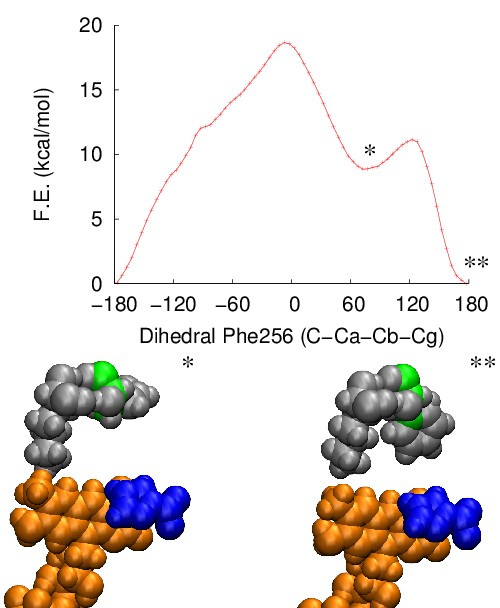
\includegraphics[width=0.5\textwidth]{msox_ph256_gate}}
+(0,-6.5) node(text1) [anchor=north west,text width=0.5\textwidth] {Substrate induces closure of Phe256 ``gate''.}
++(6.0,-1) node(image2) [graphics,anchor=north west] {
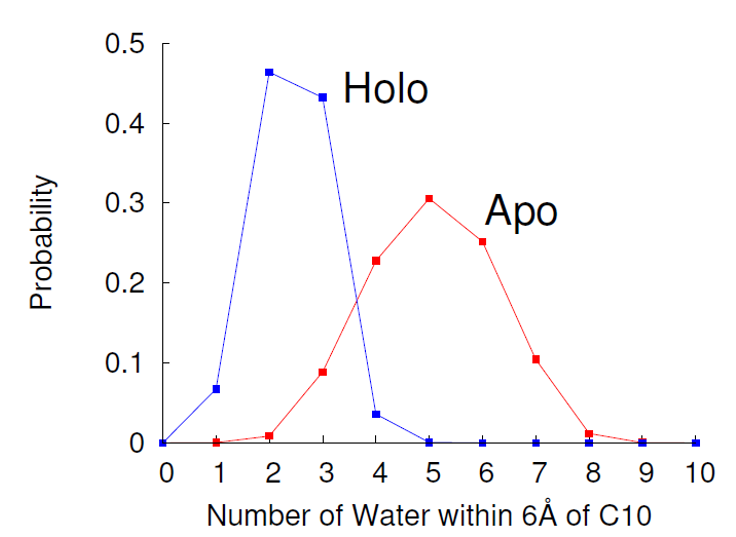
\includegraphics[width=0.5\textwidth]{msox_water}}
+(0,-4) node(text2) [anchor=north west,text width=0.5\textwidth] {Substrate pushes waters out of active site.};
\end{tikzpicture}
\end{frame}


\section{Summary}

\begin{frame}[fragile]{Summary}
\begin{itemize}
\item OTFP combines enhanced sampling and free-energy-profile generation to provide deeper understanding of biomolecular mechanisms
\item We recapitulate water-mediated ``knock-on'' transport of multiple K$^+$ ions in Kv1.2, but also predict reduced barriers for dry transport
\item Demonstrated Markovian milestoning along minimum free-energy pathways to estimate entry and exit rates of O$_{\sf 2}$ in MSOX
\item MSOX: Simulations agree with experiment that modified ping-pong mechanism is more likely than ping-pong because substrate influences O$_{\sf 2}$
entry and exit kinetics
\item MSOX: Substrate-induced gatekeeper closing and active-site desolvation likely underly the substrates effect on O$_{\sf 2}$.
\end{itemize}
\end{frame}

\tikzstyle{startstop} = [rectangle, rounded corners, minimum width=2cm, minimum height=1.8cm,text centered, draw=black, fill=red!30]
\tikzstyle{io} = [trapezium, trapezium left angle=70, trapezium right angle=110, minimum width=1cm, minimum height=0.5cm, text centered, draw=black, fill=blue!30]
\tikzstyle{process} = [rectangle, minimum width=1cm, minimum height=1cm, text centered, draw=black, fill=orange!30]
\tikzstyle{decision} = [diamond, minimum width=1cm, minimum height=1cm, text centered, draw=black, fill=green!30, aspect=2]
\tikzstyle{myarrow} = [thick,->,>=stealth]

\begin{frame}[fragile]{Acknowledgments}
\begin{tikzpicture}[scaleall=1.0,node distance=1cm]
    \node (OTFP) [startstop, text width=4.75cm] {
            \begin{tabular}{c}OTFP/TAMD\\{\bf Prof. S. Alexis PAZ}\end{tabular}
            };
    \node (Milestoning) [startstop, text width=4.75cm,right of=OTFP,fill=blue!30,xshift=4.5cm] {\begin{tabular}{c}Milestoning\\{\bf Anthony BUCCI}\end{tabular}};
    \node (ClimbingString) [startstop, text width=4.75cm,below of=OTFP,fill=green!30,yshift=-1.4cm] {\begin{tabular}{c}Climbing Strings\\{\bf Dr. Gourav SHRIVASTAV}\end{tabular}};
    \node (Funding) [startstop, text width=4.75cm,below of=Milestoning,fill=yellow!30,yshift=-1.4cm] {\begin{tabular}{c}Funding\\NIH R01GM100472\\NSF DMR1207389\end{tabular}};
    \node (Resources) [startstop, text width=10.25cm,below of=ClimbingString,fill=orange!30,xshift=2.75cm,yshift=-1.5cm] {\begin{tabular}{c}Github Repositories\\{\tt cameronabrams/cfacv}\\{\tt cameronabrams/otfp}\\{\tt cameronabrams/pestifer}\end{tabular}};
% \pcuad{\textwidth}{\textheight}
%\showcuad
% \path(nw) ++(-0.5,0.0) node(text1) [anchor=north west,text width=1.1\textwidth,execute at begin node=\setlength{\baselineskip}{1em}]{
% Projects in this talk:
% \begin{itemize}
% \item {\bf OTFP/TAMD:}  \textcolor{red}{Prof. S. Alexis PAZ} (N. U. C\'ordoba, Argentina)
% \item {\bf Milestoning:}  \textcolor{blue}{Anthony BUCCI} (PhD, 2016) (West Pharma)
% \item {\bf Climbing String:} \textcolor{blue}{Dr. Gourav SHRIVASTAV}
% \item {\bf Other current/recent projects:}
% \begin{itemize}
%     \item HIV-1 Envelope Spike Glycoprotein Conformational Dynamics: Salabil ABOU-HATAB
%     \item HIV-1 Entry Inhibitor Design:
%     \begin{itemize}
%         \item Steven GOSSERT (PhD, 2021)
%         \item Natasha VERGARA (PhD, 2022)
%         \item Dr. Mohammadjavad MOHAMMADI (2023)
%     \end{itemize}
%     \item  Molecular modeling of thermosets
%     \begin{itemize}
%         \item Ming HUANG (2023)
%         \item Dr. Salman ZARRINI (2022, Honeywell)
%     \end{itemize}
% \end{itemize}
% \item {\bf Collaborators}
% \begin{itemize}
%     \item \textcolor{green!80!black}{Prof. S. Alexis PAZ} (N. U. C\'ordoba, Argentina)
%     \item \textcolor{green!80!black}{Prof. Eric VANDEN-EIJNDEN} (NYU)
%     \item Prof. Irwin CHAIKEN (Drexel Med)
%     \item Prof. Walther MOTHES (Yale)
%     \item Prof. Joseph SODROSKI (Dana Farber Cancer Institute)
% \end{itemize}
% \end{itemize}
% \begin{itemize}
% \item {\bf Funding (this talk):} NIH R01GM100472, NSF DMR1207389
% \item {\bf Resources:} {\tt www.github.com/cameronabrams/cfacv}, {\tt www.github.com/cameronabrams/pestifer}
% \end{itemize}
% };
\end{tikzpicture}
\end{frame}
  

\end{document}
